\documentclass[11pt]{article}
\usepackage[T1]{fontenc}
\usepackage[utf8]{inputenc}
\usepackage{fourier}
\usepackage[scaled=0.875]{helvet}
\renewcommand{\ttdefault}{lmtt}
\usepackage{amsmath,amssymb}
\usepackage{makeidx}
\makeindex
\usepackage{fancybox}
\usepackage[normalem]{ulem}
\usepackage{pifont}
\newcommand{\textding}[1]{\text{\ding{#1}}}
\usepackage{lscape}
\usepackage{tabularx,booktabs}
\usepackage{scratch3}
\usepackage{textcomp}
\usepackage{enumitem}
\usepackage{multicol}
\usepackage{multirow}
\definecolor{scrmovedddd}{HTML}{3373cc}%
\newcommand{\euro}{\eurologo{}}
%Tapuscrit : Denis Vergès 
\usepackage{pst-eucl}
\usepackage{diagbox}% à mettre après pst-eucl
\usepackage{graphicx,pstricks,pst-plot,pst-grad,pst-node,pst-text,pstricks-add}
\usepackage{pstricks-add}
\usepackage{pgf,tikz,pgfplots}
\usetikzlibrary{patterns,calc,decorations.pathmorphing}
\newcommand{\R}{\mathbb{R}}
\newcommand{\N}{\mathbb{N}}
\newcommand{\D}{\mathbb{D}}
\newcommand{\Z}{\mathbb{Z}}
\newcommand{\Q}{\mathbb{Q}}
\newcommand{\C}{\mathbb{C}}
\usepackage[left=3.5cm, right=3.5cm, top=2.2cm, bottom=2cm]{geometry}
\setlength\headheight{13.7pt}
\newcommand{\vect}[1]{\overrightarrow{\,\mathstrut#1\,}}
\renewcommand{\theenumi}{\textbf{\arabic{enumi}}}
\renewcommand{\labelenumi}{\textbf{\theenumi.}}
\renewcommand{\theenumii}{\textbf{\alph{enumii}}}
\renewcommand{\labelenumii}{\textbf{\theenumii.}}
\def\Oij{$\left(\text{O}~;~\vect{\imath},~\vect{\jmath}\right)$}
\def\Oijk{$\left(\text{O}~;~\vect{\imath},~\vect{\jmath},~\vect{k}\right)$}
\def\Ouv{$\left(\text{O}~;~\vect{u},~\vect{v}\right)$}
\usepackage{fancyhdr}
\usepackage[french]{babel}
\usepackage[np]{numprint}
\usepackage{colortbl}
%\usetikzlibrary{backgrounds}
%\usetikzlibrary{calc,shapes.arrows,decorations.pathreplacing}

\usepackage[dvips,colorlinks=true,linkcolor=blue,citecolor=blue,urlcolor=blue]{hyperref}
\hypersetup{%
pdfauthor = {APMEP},
pdfsubject = {Brevet},
pdftitle = {Année 2023},
allbordercolors = white,
pdfstartview=FitH}

\begin{document}
\setlength\parindent{0mm}
\rhead{\textbf{A. P{}. M. E. P{}.}}
\lhead{\small L'intégrale 2023}

\pagestyle{fancy}
\thispagestyle{empty}
\begin{center} {\Large \textbf{\decofourleft~Brevet des collèges 2023~\decofourright\\\vspace{1cm} L'intégrale de mai 2023 à décembre 2023}}

\vspace{1cm}

Pour un accès direct cliquez sur les liens {\Large \textcolor{blue}{bleus}}
\end{center}

\phantomsection 
 \label{sommaire}
 \hypertarget{sommaire}{}
 
\begin{tabularx}{\linewidth}{>{\Large}X}

\hyperlink{AmeriqueduNord}{Amérique du Nord - 31 mai 2023}\dotfill \pageref{AmeriqueduNord} \\
\hyperlink{Etranger}{Centres étrangers - 14 juin 2023} \dotfill \pageref{Etranger} \\
\hyperlink{Asie}{Asie - 19 juin 2023} \dotfill \pageref{Asie} \\
\hyperlink{Polynesie}{Polynésie - 23 juin 2023} \dotfill \pageref{Polynesie} \\
\hyperlink{Metropole}{Métropole, La Réunion, Antilles-Guyane - 26 juin 2023} \dotfill \pageref{Metropole}\\
\hyperlink{Polynesiesep}{Polynésie 11 septembre 2023} \dotfill \pageref{Polynesiesep} \\
\hyperlink{Metropolesep}{Métropole, La Réunion, Antilles--Guyane 18 sept. 2023} \dotfill \pageref{Metropolesep} \\
\hyperlink{AmeriqueSud}{Amérique du Sud 16 novembre 2023}  \dotfill \pageref{AmeriqueSud} \\
\hyperlink{Caledoniedec}{Nouvelle-Calédonie 7 décembre 2023}  \dotfill \pageref{Caledoniedec}
\end{tabularx}

\vspace{1cm}

\hyperlink{Index}{À la fin index des notions abordées}


\newpage
 ~
\newpage
%%%%%%%%   Amérique du Nord 31 mai 2023

\rhead{\textbf{A. P{}. M. E. P{}.}}
\lhead{\small Brevet des collèges}
\rfoot{\small{Amérique du Nord}}
\lfoot{\small{31 mai 2023}}
	\pagestyle{fancy}
	\thispagestyle{empty}

 \phantomsection
 
\hypertarget{AmeriqueduNord}{}
\label{AmeriqueduNord}

	\begin{center}\textbf{Durée : 2 heures}
{\Large\textbf{\decofourleft~Diplôme national du Brevet
Amérique du Nord~\decofourright}}\\[7pt]
{\Large \textbf{31 mai 2023}}

%\medskip
%		\emph{L'usage de calculatrice avec mode examen activé est autorisé.\\
%			L'usage de calculatrice sans mémoire \og type collège \fg{} est autorisé}
%
%
%Le sujet est constitué de cinq exercices indépendants.
%
%Le candidat peut les traiter dans l'ordre qui lui convient.
%
%Indication portant sur l'ensemble du sujet. Toutes les réponses doivent être justifiées, sauf si une indication contraire est donnée. Pour chaque question, si le travail n'est pas terminé, laisser une trace de la recherche elle sera prise en compte dans la notation.
\end{center}

\vspace{0,5cm}

\textbf{{\large \textsc{Exercice 1}} \hfill 20 points}

\medskip
\emph{\textbf{Les cinq situations suivantes sont indépendantes.}}

\bigskip

\textbf{Situation 1}

Décomposer en produit de facteurs premiers le nombre 780.\index{Produit de facteurs premiers}

\emph{Aucune justification n'est attendue.}

\bigskip

\textbf{Situation 2}

On rappelle qu'un jeu de 32 cartes est composé de quatre familles (trèfle, carreau, cœur, pique). Chaque famille est composée de huit cartes : $7,8,9,10$, valet, dame, roi et as.

L'expérience aléatoire consiste à tirer une carte au hasard dans ce jeu de 32 cartes.

\begin{enumerate}
	\item Quelle est la probabilité d'obtenir le 8 de pique ? \emph{Aucune justification n'est attendue.}
	\item Quelle est la probabilité d'obtenir un roi ou un cœur ? \emph{Aucune justification n'est attendue.}\index{Probabilité}
\end{enumerate}

\bigskip

\textbf{Situation 3}

Développer et réduire l'expression $A$.

$A=(2 x + 5)(3 x - 4)$\index{Développement}


\begin{minipage}{0.5\linewidth}
\bigskip

\textbf{Situation 4}

\begin{enumerate}
	\item Quel est le volume, en $\mathrm{cm}^{3}$, de ce prisme droit ?
	\item Convertir ce résultat en litre.

	Rappel : $\np[L]{1}=\np[dm^{3}]{1}$\index{Volume prisme}
\end{enumerate}
\end{minipage}
\hfill
\begin{tikzpicture}[>=stealth,baseline={(current bounding box.center)}]
	\draw[line width=1pt] (0,0)--(5,0)--(7.2,2.1)--(2.2,4.4)--(0,2.3)--cycle (0,2.3)--(5,0) (0.35,0)--(0.35,0.35)--(0,0.35);
	\draw[line width=1pt,dash pattern=on 2mm off 1.5mm] (2.2,2.1)--(0,0) (2.2,2.1)--(7.2,2.1) (2.2,2.1)--(2.2,4.4) (2.55,2.1)--(2.55,2.45)--(2.2,2.45);
	\draw[<->] (0,-0.2)--(5,-0.2) node[midway, below]{\np[cm]{80}} ;
	\draw[<->] (-0.2,0)--(-0.2,2.3) node[midway, above, sloped]{\np[cm]{60}} ;
	\draw[<->] (5.1,-0.1)--(7.3,2.) node[midway, below, sloped]{\np[cm]{120}} ;
	\draw[<->] (7.25,2.25)--(2.25,4.55) node[midway, above, sloped]{\np[cm]{100}} ;
\end{tikzpicture}

\begin{minipage}[t]{0.5\linewidth}
\textbf{Situation 5}

Le polygone 2 est un agrandissement du polygone 1.

Le coefficient de cet agrandissement est 3.

L'aire du polygone 1 est égale à $\np[cm^2]{11}$.\index{Agrandissement}

	\medskip

Quelle est l'aire du polygone 2 ?

\end{minipage}
\hfill
\begin{tikzpicture}[baseline={(T.base)}]
	\node[align = left, text width=65mm, below right] (T) at (0.2,5.8){Représentation de la situation qui n'est pas à l'échelle :};
	\draw (0,0) rectangle (7,6);
	\draw[line width = 1pt, fill = lightgray, shift={(1,2)}] (0,0)--(0.7,0.22)--(0.5,0.7)--(0,1)--(-0.5,0.4)--cycle;
	\draw[line width = 1pt, fill = lightgray, shift={(4.5,1.3)}] (0,0)--(2.1,0.66)--(1.5,2.1)--(0,3)--(-1.5,1.2)--cycle ;
	\node (Pun) at (1,0.5){Polygone 1};
	\node (Pdeux) at (4.5,0.5){Polygone 2};
\end{tikzpicture}

\newpage

\textbf{{\large \textsc{Exercice 2}} \hfill 22 points}

\medskip
\begin{minipage}{0.5\linewidth}
On considère la figure ci-contre.

On donne les mesures suivantes :

\begin{itemize}[label=$\bullet$]
\item $\mathrm{AN}= \np[cm]{13}$

\item $\mathrm{LN}= \np[cm]{5}$

\item $\mathrm{AL} = \np[cm]{12}$

\item $\mathrm{ON}= \np[cm]{3}$

\item O appartient au segment [LN]

\item $\mathrm{H}$ appartient au segment [NA]

\end{itemize}
\end{minipage}
\hfill
\begin{tikzpicture}[baseline={(current bounding box.center)}]
		\draw[line width=1pt] (0,0)node[below left]{L}--
			(4.2,0) node[below right]{N}--
			(0,7.5) node[above left]{A} --cycle
			(1.5,0) node[below] {O}--
			(1.5,4.82) node[above right]{H}
			(1.85,0)--(1.85,0.35)--(1.5,0.35);

\end{tikzpicture}
\begin{enumerate}
\item Montrer que le triangle LNA est rectangle en L.\index{Réciproque de Pythagore}\index{Pythagore!réciproque}
\item Montrer que la longueur $\mathrm{OH}$ est égale à $7,2 \mathrm{~cm}$.\index{Thalès}
\item Calculer la mesure de l'angle $\widehat{\mathrm{LNA}}$. Donner une valeur approchée à l'unité près.\index{Trigonométrie}
\item Pourquoi les triangles LNA et ONH sont-ils semblables ?
\item 
	\begin{enumerate}
		\item Quelle est l'aire du quadrilatère LOHA ?
		\item Quelle proportion de l'aire du triangle LNA représente l'aire du quadrilatère LOHA ?
	\end{enumerate}
\end{enumerate}

\vspace{0,5cm}

\textbf{{\large \textsc{Exercice 3}} \hfill 20 points}

\medskip

\textbf{\emph{Les deux parties sont indépendantes.}}

\medskip

\textbf{Partie A : Évolution du nombre de visiteurs sur un site touristique.}
\begin{enumerate}
\item Le diagramme ci-dessous représente le nombre de visiteurs par an de 2010 à 2021 sur ce site.


\begin{tikzpicture}[scale=0.85] %pour l'échelle proche du sujet original : scale=1 (ou supprimer l'option)
	\node[] at(7,5) {Nombre de visiteurs sur le site touristique par année};
	\draw[gray,xstep = 14,ystep = 0.5](-0.1,0) grid (14,4.5);
	\foreach \y in {5,10,...,45}{\node at (-0.2,{\y/10}) [left] {$\np{\y0000}$};}
	\node at (-0.2,0) [left] {$\np{0}$};
	\node[rotate=90] at(-2,2.25)  {Nombre de visiteurs};
	\foreach \x/\y/\a in {0/3/2010,1/3.1/2011,2/3.2/2012,3/3.2/2013,4/3.15/2014,5/3.3/2015,6./3.35/2016,7/3.48/2017,8/3.55/2018,9/4.1/2019,10/1.87216/2020,11/2.19042/2021}{\draw[fill=gray] ((0.3+1.15*\x,\y) rectangle (0.8+1.15*\x,0) ++(-0.25,0) node [below] {$\a$};}
	\node[] at(7,-0.7) {Année};
\end{tikzpicture}

	\begin{enumerate}
		\item Quel a été le nombre de visiteurs en 2010 ? \emph{Aucune justification n'est attendue.}\index{Histogramme}
		\item En quelle année le nombre de visiteurs a-t-il été le plus élevé ? \emph{Aucune justification n'est attendue.}
	\end{enumerate}

\item Le tableau ci-dessous indique le nombre de visiteurs sur le site touristique de cette ville en 2020 et en 2021 :
\begin{center}
\begin{tabular}{|l|c|c|}
\hline
Année & 2020 & 2021 \\
\hline
Nombre de visiteurs & \np{187216} & \np{219042} \\
\hline
\end{tabular}
\end{center}

Le maire de cette ville avait pour objectif que le nombre de visiteurs progresse d'au moins $15\,\%$ entre 2020 et 2021.\index{Pourcentage}

L'objectif a-t-il été atteint ?
\end{enumerate}

\medskip

\textbf{Partie B : Étude des prix des hôtels de cette ville.}

\smallskip

Sur une période donnée, on relève les prix facturés pour une nuit par les hôtels de cette ville.

\begin{center}
\begin{tabular}{|l|c|c|c|c|c|c|c|c|}
\hline
$\begin{array}{@{}l}\text { Prix facturés pour } \\ \text { une nuit (en euro) }\end{array}$ & 60 & 80 & 85 & 90 & 110 & 120 & 350 & 500 \\ \hline
Effectif & \np{1200} & \np{1350} & \np{1000} & \np{1100} & \np{1200} & \np{1300} & 900 & 300 \\ \hline
\end{tabular}
\end{center}

\begin{enumerate}
\setcounter{enumi}{2}
\item Déterminer l'étendue des prix facturés.\index{Etendue@Étendue}
\item Quelle est la moyenne des prix facturés pour une nuit ? Arrondir à l'euro près.\index{Moyenne}
\item L'association des hôteliers de cette ville cherche à attirer des touristes et annonce : \og Dans les hôtels de notre ville, au moins la moitié des nuits est facturée à moins de $100 $\,\euro{} \fg. Est-ce vrai ?
\end{enumerate}

\vspace{0,5cm}

\textbf{{\large \textsc{Exercice 4}} \hfill 20 points}

\medskip

À l'aide d'un logiciel de programmation, on veut réaliser le motif \og Fleur \fg{} suivant.

\begin{center}
\begin{tikzpicture}[]
	\node at(0,2) {\textbf{Motif \og Fleur »}};
	\foreach \a in {0,...,4}
	{\draw[line width = 1pt,rotate=72*\a] (0,0)--(0.9,0)-- ++(60:0.45)-- ++(-0.9,0)--cycle ;}
	\draw (-2.5,-2.3) rectangle (2.5,2.3);
	\draw[>=stealth,<-] (-0.3,-0.5)--(-1.5,-1.3) node[below] {Un pétale};
\end{tikzpicture}
\end{center}

\begin{enumerate}
\item
	\begin{enumerate}
		\item Le parallélogramme KLMN ci-dessous représente un des pétales du motif \og Fleur\fg.
		
Construire ce parallélogramme sur la copie en prenant $1 \mathrm{~cm}$ pour 5 pas.
%\begin{center}
%\begin{tikzpicture}[]
%  			\draw[line width = 1pt] (0,0)node[below left]{K}--(5,0) node[below right]{L}-- ++(60:3.5)node[above right] {M}-- ++(-5,0) node[above left] {N}--cycle ;
%  			\draw[line width = 1pt, shift={(5,0)} ] (-0.45,0) arc (180:60:0.45)node[pos=0.6, above left]{120\textdegree}  ;
%  			\draw[line width = 1pt, shift={(5,0)} ] (60:3.5)++(-0.55,0) arc (180:240:0.55)node[pos=0.6,below left]{60\textdegree}  ;
%  		\end{tikzpicture}
%\end{center}
\begin{center}
\psset{unit=0.8cm}
\begin{pspicture}(9.5,4)
\pspolygon(0.2,0.4)(7.2,0.4)(9.2,3.8641)(2.2,3.8641)
\uput[dl](0.2,0.4){K} \uput[dr](7.2,0.4){L} \uput[ur](9.2,3.8641){M} \uput[ul](2.2,3.8641){N} \uput[d](3.7,0.4){35 pas} \uput[ul](7,0.6){$120\degres$} \uput[dl](9,3.6641){$60\degres$} \uput[r](8.2,2.13){20 pas} 
\psarc(7.2,0.4){0.5}{60}{180}\psarc(9.2,3.8641){0.4}{180}{240}
\end{pspicture}
\end{center}
	\item \begin{minipage}[t]{0.6\linewidth}
On définit le bloc \og Pétale \fg{} ci-contre afin de dessiner ce parallélogramme.

On commence la construction du parallélogramme au point $\mathrm{K}$ en s'orientant vers la droite.

Par quelles valeurs doit-on compléter les lignes $4,5,6$, et 7 du bloc \og Pétale \fg{} ci-contre ?\emph{Aucune justification n'est attendue, écrire sur la copie le numéro de la ligne du bloc \og Pétale \fg{} et la valeur correspondante.}
	\end{minipage}\hfill
	\begin{tikzpicture}[baseline=(T.base)]
		\node (T) at(0,0)[below right]{\textbf{Bloc « Pétale »}};
		\node at(0,-0.5)[below right]{
		\begin{scratch}[num blocks, scale=0.8]
		\initmoreblocks{définir \namemoreblocks{Pétale}}
		\blockpen{stylo en position d'écriture}
		\blockrepeat{répéter \ovalnum{2} fois}{
		\blockmove{avancer de \ovalnum{~ ~ ~} pas}
		\blockmove{tourner \turnleft{} de \ovalnum{~ ~ ~} degrés}
		\blockmove{avancer de \ovalnum{~ ~ ~} pas}
		\blockmove{tourner \turnleft{} de \ovalnum{~ ~ ~} degrés}}
	\end{scratch} };
	\draw (-0.2,0.2)rectangle (4.7,-7.2);
\end{tikzpicture}
\end{enumerate}

\item Le bloc ci-dessous permet de construire un motif \og Fleur \fg{} en partant de son centre.\index{Scratch}

	\hfill~
	\begin{tikzpicture}[baseline=(T.base)]
		\draw (-0.2,0.2) rectangle (4.5,-5);
		\node (T) at(0,0)[below right]{\textbf{Bloc \og Fleur \fg{}}};
		\node at(0,-0.5)[below right]{
		\begin{scratch}[scale=0.8]
			\initmoreblocks{définir \namemoreblocks{Fleur}}
			\blockrepeat{répéter \ovalnum{~ ~ ~} fois}{
				\blockmoreblocks{Pétale}
				\blockmove{tourner \turnright{} de \ovalnum{72} degrés}}
		\end{scratch}};
	\end{tikzpicture}
	\hfill~
	\begin{tikzpicture}[baseline=(T.base)]
		\draw (-0.2,0.2) rectangle (4.2,-4.2);
		\node (T) at(0,0)[below right]{\textbf{Motif « Fleur »}};
		\foreach \a in {0,...,4}
		{\draw[shift={(2,-2.4)},line width = 1pt,rotate=72*\a] (0,0)--(1.05,0)-- ++(60:0.6)-- ++(-1.05,0)--cycle ;}
	\end{tikzpicture}
	\hfill~

\begin{enumerate}
	\item Par quelle valeur doit-on compléter la ligne 2 du bloc \og Fleur \fg{} ci-dessus ? \emph{Aucune justification n'est attendue.}
	\item Expliquer le choix de la valeur « 72 » dans la ligne 4 .
	\item On modifie le bloc « Fleur » pour construire le motif suivant :
	
		\hfill~
	\begin{tikzpicture}[baseline=(T.base),scale=2]
		\clip (-2,1.5) rectangle (2,-1.5);
		\foreach \a in {0,...,11}
		{\draw[line width = 1pt,rotate=30*\a] (0,0)--(1.05,0)-- ++(60:0.6)-- ++(-1.05,0)--cycle ;}
	\end{tikzpicture}
	\hfill~

	Quelles sont alors les modifications à apporter aux lignes 2 et 4 du bloc \og Fleur \fg{} ? \emph{Aucune justification n'est attendue.}
	\end{enumerate}
\end{enumerate}

\vspace{0,5cm}

\newpage

\textbf{{\large \textsc{Exercice 5}} \hfill 18 points}

\medskip

Un hippodrome est un lieu où se déroulent des courses de chevaux.

On s'intéresse à la piste d'un hippodrome.

Cette piste est composée de :

\begin{itemize}
\item deux lignes droites modélisées par des segments de $850$ mètres ;
\item deux virages modélisés par deux demi-cercles de rayon $40$ mètres.

\end{itemize}

\begin{center}
	\begin{tabular}{|c|} \hline
	Schéma de la piste de cet hippodrome :\\
	\begin{tikzpicture}[]

		\draw[line width=1pt] (0,0)--(10,0) arc (-90:90:1.4)--(0,2.8)arc (90:270:1.4);
		\draw [<->, >=stealth] (0,-0.2)--(10,-0.2)node[midway, below]{Segment de longueur : \np[m]{850}};
		\draw [<->, >=stealth] (10,2.8)--(10,1.4)node[midway, left]{Rayon : \np[m]{40}};
		\draw[dash pattern=on 1.7mm off 1.3mm] (0,0)--(0,2.8) (10,0)--(10,1.4) ;
		\clip (-2,-0.3) rectangle (12,3.2) ;

	\end{tikzpicture}
	\\ \hline
\end{tabular}
\end{center}

\begin{enumerate}
\item Montrer que la longueur d'un tour de piste est d'environ $\np{1951} \mathrm{~m}$.\index{Longueur du cercle}
\item Un cheval parcourt un tour de piste en $2 \min 9 \mathrm{~s}$.
	\begin{enumerate}
		\item Calculer la vitesse moyenne de ce cheval sur un tour de piste en mètre par seconde $(\mathrm{m} / \mathrm{s})$. Donner une valeur approchée à l'unité près.\index{Vitesse}

		\item Convertir cette vitesse en kilomètre par heure $(\mathrm{km} / \mathrm{h})$.
	\end{enumerate}

\item On admet que la surface de la piste a une aire d'environ $\np{73027} \mathrm{~m}^{2}$.

On souhaite semer du gazon sur la totalité de la surface de la piste.

On doit choisir des sacs de gazon à semer parmi les trois marques ci-dessous :

\begin{center}
\begin{tabular}{|c|c|c|}
\cline { 2 - 3 }
\multicolumn{1}{c|}{} & Surface couverte par sac & Prix d'un sac \\ \hline
Marque A & $500 \mathrm{~m}^{2}$ & $141,95$ \euro{} \\ \hline
Marque B & $400 \mathrm{~m}^{2}$ & $87,90$ \euro{} \\
\hline
Marque C & $300 \mathrm{~m}^{2}$ & $66,50$ \euro{} \\ \hline
\end{tabular}
\end{center}

Quelle marque doit-on choisir pour que cela coûte le moins cher possible ?
\end{enumerate}

\hyperlink{sommaire}{Retour au sommaire}
%%%%%%%%%   fin Amérique du Nord 31 mai 2023
\newpage
%%%%%%%%%   Étranger 14 juin 2023

\rfoot{\small Centres étrangers Groupe I}
\lfoot{\small 14 juin 2023}
\pagestyle{fancy}
\thispagestyle{empty}

 \phantomsection

\label{Etranger}
\hypertarget{Etranger}{}

\begin{center} {\Large \textbf{\decofourleft~Brevet Centres étrangers Groupe I - 14 juin 2023 \decofourright}}
\end{center}

\bigskip

\textbf{Exercice 1 \hfill 18 points}

\medskip

Cet exercice, en deux parties, est un questionnaire à choix multiples (QCM). Pour chaque question, parmi les réponses proposées, une seule est exacte. Recopier le numéro de la question et indiquer la réponse choisie.

\textbf{Aucune justification n'est attendue ici}

\medskip

\textbf{Partie A}

\medskip

Dans cette partie, on s'intéresse au programme ci-dessous, composé d'un bloc \og triangle équilatéral\fg{} et d'un script principal:

\begin{center}
\begin{tabular}{m{6.5cm}|m{6.5cm}}
Bloc \og triangle équilatéral\fg 	&Script principal\\
\begin{scratch}
\initmoreblocks{définir \namemoreblocks{triangle équilatéral}}
\blockpen{stylo en position d’écriture}
\blockrepeat{répéter \ovalnum{3} fois}
{\blockmove{avancer de \ovalnum{50} pas}
\blockmove{tourner \turnleft{} de \ovalnum{} degrés}
}
\end{scratch}						&\begin{scratch}

\blockmove{aller à x: \ovalnum0 y: \ovalnum0}
\blockmove{s’orienter à \ovalnum{90} degrés}
\blockpen{effacer tout}
\blockrepeat{répéter \ovalnum{2} fois}
{
\blockpen{stylo en position d’écriture}
\blockmoreblocks{triangle équilatéral}
\blockpen{relever stylo}
\blockmove{tourner \turnleft{} de \ovalnum{60} degrés}
}
\end{scratch}\\
&On rappelle que l'instruction \og s'orienter à 90 \fg{} signifie s'orienter vers la droite.\\
\end{tabular}

\smallskip
\begin{tabularx}{\linewidth}{|m{5cm}|*{3}{>{\centering \arraybackslash}X|}}\hline
Questions&Réponse A&Réponse B&Réponse C\\ \hline
\textbf{1.} On souhaite construire le triangle équilatéral ci-dessous.

Le stylo est orienté à $90\degres$ au départ comme ci-dessous.\index{Scratch}

Départ\begin{pspicture}(-0.5,-0.1)(2.,1.6)
\psline{->}(-0.5,0)(0,0)
\pspolygon(0;0)(1.7;0)(1.7;60)
\psdots(0.85;0)(1.472;30)(0.85;60)
\end{pspicture}

Compléter le script du bloc \og triangle équilatéral \fg{} avec la valeur qui convient.&$60\degres$&$100\degres$&$120\degres$\\ \hline
\textbf{2.} Parmi les trois figures, laquelle est obtenue avec le script principal ?&\psset{unit=1cm}
\begin{pspicture}(-1,0)(1.3,1.4)
\def\tri{\pspolygon(0;0)(1.2;0)(1.2;60)}
\rput(0,0){\tri}\rput{90}(0,0){\tri}
\end{pspicture} & \psset{unit=1cm}
\begin{pspicture}(-1.3,0)(1.3,1.4)
\def\tri{\pspolygon(0;0)(1.2;0)(1.2;60)}
\rput(0,0){\tri}\rput(-1.2,0){\tri}
\end{pspicture}&\psset{unit=1cm}
\begin{pspicture}(-1,0)(1.3,1.4)
\def\tri{\pspolygon(0;0)(1.2;0)(1.2;60)}
\rput(0,0){\tri}\rput{60}(0,0){\tri}
\end{pspicture}\\ \hline
\textbf{3.} Quel polygone obtient-on si on remplace dans le script principal, la boucle \og répéter 2 fois \fg{} par une boucle \og  répéter 6 fois \fg{} ?&Un parallélogramme
&Un hexagone
&Un losange\\ \hline
\end{tabularx}
\end{center}

\medskip

\textbf{Partie B}

\medskip

\begin{tabularx}{\linewidth}{|m{6.5cm}|*{3}{>{\centering \arraybackslash}X|}}
\hline
Questions&Réponse A&Réponse B&Réponse C\\ \hline
\textbf{1.} $\left(\dfrac23 - \dfrac13 \times\dfrac75\right) \div \dfrac 43 = $&$\dfrac{3}{15} \times \dfrac43$&$\left(\dfrac13 \times \dfrac75 \right) \div \dfrac43$&$\dfrac{3}{15} \times \dfrac34$\rule[-11pt]{0pt}{30pt}\\ \hline\index{Calcul numérique}
\textbf{2.} L'écriture scientifique de $302,4 \times 10^{18}$ est:&$3,024 \times 10^{16}$&$3,024 \times 10^{20}$&$\np{0,3024} \times 10^{21}$\\ \hline\index{Ecriture scientifique@Écriture scientifique}
\textbf{3.} On donne ci-dessous la masse de 8 biscuits différents:

12 g ; 10 g ; 18 g ; 8 g ; 12 g ; 15 g ; 11 g ; 13 g

Suite à une erreur de mesure, le biscuit pesant 18 g pèse en fait 16 g.

Une fois cette erreur corrigée, la valeur de la médiane sera : & Plus petite. & La même. & Plus grande.\\ \hline 
\end{tabularx} \index{Médiane}

\bigskip

\textbf{Exercice 2 \hfill 24 points}

\medskip

\emph{Les trois parties de cet exercice sont indépendantes et peuvent être traitées séparément.}

\medskip

Une famille souhaite installer dans son jardin une cabane.

La partie inférieure de cette cabane est modélisée par le rectangle BCDF:

\begin{center}
\psset{unit=1cm}
\begin{pspicture}(10,3.2)
\pspolygon(0,0.2)(9.5,0.2)(5.6,2.5)(1.4,2.5)%AEFB
\psline(5.6,2.5)(5.6,0.2)%FD
\psline(1.4,2.5)(1.4,0.2)%BC
\psline[linestyle=dashed](1.4,1)(0.45,1)%NM
\psframe(1.4,1)(1.2,1.2)\psframe(1.4,0.2)(1.2,0.4)\psframe(5.6,0.2)(5.8,0.4)
\psarc(9.5,0.2){0.6}{150}{180}
\uput[d](0,0.2){A} \uput[d](1.4,0.2){C} \uput[d](5.6,0.2){D} \uput[dr](9.5,0.2){E} 
\uput[u](5.6,2.5){F} \uput[u](1.4,2.5){B} \uput[d](1.4,0.2){C} \uput[r](1.4,1){N}
\uput[ul](0.45,1){M}
\rput(8.7,3){Toboggan}\rput(0.7,3.1){Escalier}
\psline{->}(8.7,2.8)(7.4,1.43)
\psline{->}(0.6,2.9)(0.8,1.57)
\end{pspicture}
\end{center}

On précise que:

\begin{center}
\begin{tabularx}{\linewidth}{m{4.5cm} X}
$\bullet~$AB = 1,3 m ;&$\bullet~$DE = 2,04 m ;\\
$\bullet~$AC = 0,5 m ;&$\bullet~$Les triangles ABC, BMN et FDE sont rectangles.\\
$\bullet~$BC = DF = 1,2 m ;&\\ 
\end{tabularx}
\end{center}

\textbf{Partie A: Étude du toboggan}

\medskip

\begin{enumerate}
\item Pour que le toboggan soit sécurisé, il faut que l'angle $\widehat{\text{DEF}}$ mesure $30\degres$, au degré près.

Le toboggan de cette cabane est-il sécurisé ?\index{Trigonométrie}
\item Montrer que la rampe du toboggan, EF, mesure environ $2,37$~m.\index{Pythagore}
\end{enumerate}

\medskip

\textbf{Partie B : Étude de l'échelle}

\medskip

Pour consolider l'échelle, on souhaite ajouter une poutre supplémentaire [MN], comme indiqué sur le modèle.

\medskip

\begin{enumerate}
\item Démontrer que les droites (AC) et (MN) sont parallèles.
\item On positionne cette poutre [MN] telle que BN = 0,84 m. Calculer sa longueur MN.\index{Thalès}
\end{enumerate}

\medskip

\textbf{Partie C : Étude du bac à sable}

\medskip

Un bac à sable est installé sous la cabane. Il s'agit d'un pavé droit dont les dimensions sont :

$\bullet~$Longueur : 200 cm

$\bullet~$Largeur : 180 cm

$\bullet~$Hauteur : 20 cm

\medskip

\begin{enumerate}
\item Calculer le volume de ce bac à sable en cm$^3$.\index{Volume du pavé}
\item On admet que le volume du bac à sable est de $0,72$~m$^3$.

On remplit entièrement ce bac avec un mélange de sable à maçonner et de sable fin dans le ratio 3 : 2.

Vérifier que le volume nécessaire de sable à maçonner est de $0,432$ m$^3$ et que celui de sable fin est de $0,288$~m$^3$.
\item Un magasin propose à l'achat le sable à maçonner et le sable fin, vendus en sac. D'après les indications ci-dessous, quel est le coût total du sable nécessaire pour remplir entièrement ce bac à sable sachant qu'on ne peut acheter que des sacs entiers ?

\begin{center}
\begin{tabular}{l |l}
Un  sac de sable à maçonner:& Un sac de sable fin:\\
Poids : 35 kg&Poids : 25 kg\\
Volume : 0,022~m$^3$&Volume : 0,016~m$^3$\\
Prix : 2,95~\euro&Prix : 5,95~\euro\\
\end{tabular}
\end{center}
\end{enumerate}

\bigskip

\textbf{Exercice 3 \hfill 15 points}

\medskip

Amir et Sonia ont chacun inventé un programme de calcul.\index{Programme de calcul}

\begin{center}
\begin{tabularx}{\linewidth}{X X}
Programme d'Amir&Programme de Sonia\\
$\bullet~~$Choisir un nombre &$\bullet~~$Choisir un nombre \\
$\bullet~~$Soustraire 5&$\bullet~~$Ajouter 3\\
$\bullet~~$Prendre le double du résultat&$\bullet~~$ Multiplier le résultat par le nombre choisi\\
 &$\bullet~~$ Soustraire 16
\end{tabularx}
\end{center}

\begin{enumerate}
\item Montrer que si le nombre choisi au départ est 6 alors on obtient 2 avec le programme d'Amir et on obtient 38 avec celui de Sonia.
\item Amir et Sonia souhaitent savoir s'il existe des nombres choisis au départ pour lesquels les deux programmes renvoient le même résultat.

Pour cela, ils complètent la feuille de calcul ci-dessous :

\begin{center}
\begin{tabularx}{\linewidth}{|c|l|*{7}{>{\centering \arraybackslash}X|}}\hline
&A&B &C&D &E &F &G &H\\ \hline
1&Nombre choisi&$-2$&$-1$&0&1&2&3&4\\ \hline
2&Programme d'Amir&$-14$& $-12$& $-10$& $-8$& $-6$& $-4$& $-2$\\ \hline
3&Programme de Sonia& $-18$ &$-18$ &$-16$ &$-12$ &$-6$ &$2$ &$12$\\ \hline
\end{tabularx}
\end{center}

\emph{Aucune justification n'est attendue pour les deux questions ci-dessous.}

\medskip

	\begin{enumerate}
		\item Parmi les trois propositions suivantes, recopier sur votre copie la formule qui a été saisie dans la cellule B2 avant d'être étirée vers la droite.\index{Tableur}
\begin{center}
\begin{tabularx}{\linewidth}{*{2}{>{\centering \arraybackslash}X|}>{\centering \arraybackslash}X}
=(B1 $- 5)* 2$ &=($- 2- 5)*2$ &=B1 $- 5*2$
\end{tabularx}
\end{center}

		\item En vous aidant de la feuille de calcul, quel nombre doivent-ils choisir pour obtenir des résultats égaux avec les deux programmes?
	\end{enumerate}
\item Sonia et Amir souhaitent vérifier s'il existe d'autres nombres permettant d'obtenir des résultats égaux avec les deux programmes.

Pour cela, ils décident d'appeler $x$ le nombre choisi au départ de chacun des programmes.
	\begin{enumerate}
		\item Montrer que le résultat obtenu avec le programme de Sonia est donné par 
		
$x^2 + 3x - 16$.\index{Calcul littéral}
		\item On admet que les programmes donnent le même résultat si on choisit comme nombre de départ les solutions de l'équation $(x - 2)(x + 3) = 0$.
		
Résoudre cette équation et en déduire les valeurs pour lesquelles les deux programmes de calcul
renvoient le même résultat.
	\end{enumerate}
\end{enumerate}

\bigskip

\textbf{Exercice 4 \hfill 22 points}

\medskip

Des élèves organisent, pour leur classe, un jeu au cours duquel il est possible de gagner des lots. Pour cela, ils placent dans une urne trois boules noires numérotées de 1 à 3, et quatre boules rouges numérotées de 1 à 4, toutes indiscernables au toucher.

\bigskip

\textbf{Partie A : étude du jeu}

\medskip

\begin{enumerate}
\item On pioche au hasard une boule dans l'urne.
	\begin{enumerate}
		\item Quelle est la probabilité de tirer une boule rouge ?\index{Probabilité}
		\item Quelle est la probabilité de tirer une boule dont le numéro est un nombre pair ?
	\end{enumerate}
\item Le jeu consiste à piocher, dans l'urne, une première boule, la remettre dans l'urne puis en piocher une seconde.

Pour chacune des boules tirées, on note la couleur ainsi que le numéro.

Pour gagner un lot, il faut tirer la boule rouge numérotée 1 et une boule noire.

Quelle est la probabilité de gagner?
\end{enumerate}

\bigskip

\textbf{Partie B : constitution des lots}

\medskip

Pour constituer les lots, on dispose de $195$ figurines et $234$ autocollants.

Chaque lot sera composé de figurines ainsi que d'autocollants.

Tous les lots sont identiques.

Toutes les figurines et tous les autocollants doivent être utilisés.

\medskip

\begin{enumerate}
\item Peut-on faire 3 lots ?
\item Décomposer 195 en produit de facteurs premiers.\index{Produit de facteurs premiers}
\item Sachant que la décomposition en produit de facteurs premiers de $234$ est $2 \times 3^2 \times 13$ :
	\begin{enumerate}
		\item Combien de lots peut-on constituer au maximum ?\index{Plus grand commun diviseur}
		\item De combien de figurines et d'autocollants sera alors composé chaque lot ?
	\end{enumerate}
\end{enumerate}

\bigskip

\textbf{Exercice 5 \hfill 21 points}

\medskip

Pour se promener le long d'un canal, deux sociétés proposent une location de bateaux électriques.

Les bateaux se louent pour un nombre entier d'heures.

\medskip

\begin{enumerate}
\item \textbf{Étude du tarif proposé par la société A}

\medskip

Pour la société A, le prix à payer en fonction de la durée de location en heure est donné par le graphique en ANNEXE.

Répondre aux questions ci-dessous à l'aide du graphique.

Aucune justification n'est attendue pour les questions a. et b.
	\begin{enumerate}
		\item Quel prix va-t-on payer en louant un bateau pour 2 heures ?\index{Fonction linéaire}
		\item On dispose d'un budget de $100$~\euro, combien d'heures entières peut-on louer un bateau ?
		\item Expliquer pourquoi le prix est proportionnel à la durée de location.
		\item En déduire à l'aide d'un calcul, le prix à payer pour une durée de location de 10 heures.
	\end{enumerate}
\item \textbf{Étude du tarif proposé par la société B}

\medskip

La société B propose le tarif suivant : $60$~\euro{} de frais de dossier plus $15$~\euro{} par heure de location.
	\begin{enumerate}
		\item Montrer qu'en louant un bateau pour une durée de 2 heures, le prix à payer sera de $90$~\euro.\index{Fonction affine}
		\item On désigne par $x$ le nombre d'heures de location. On appelle $f$ la fonction qui, au nombre d'heures de location, associe le prix, en euro, avec le tarif proposé par la société B.

On admet que $f$ est définie par : $f(x) = 15x + 60$.

Sur le graphique donné en ANNEXE à rendre avec la copie, tracer la courbe représentative de la fonction $f$.
		\item Le prix payé est-il proportionnel à la durée de location ?
	\end{enumerate}
\item \textbf{Comparaison des deux tarifs}
	\begin{enumerate}
		\item On souhaite louer un bateau pour une durée de 3 heures.

Quelle société doit-on choisir pour avoir le tarif le moins cher ?

Quel prix va-t-on payer dans ce cas ?
		\item Pour quelle durée de location le prix payé est-il identique pour les deux sociétés ?
	\end{enumerate}
\end{enumerate}

\newpage
\begin{center}
\textbf{\Large ANNEXE}

\bigskip

\textbf{À compléter et à rendre avec la copie}
\end{center}

\medskip

\textbf{Exercice 5}

\bigskip

\begin{center}
\textbf{Prix payé pour la location d'un bateau en fonction de la durée de la location}

\medskip

\psset{xunit=1.4cm,yunit=0.028cm,arrowsize=2pt 3}
\begin{pspicture}(-0.5,-20)(8.25,295)
\multido{\n=0.0+0.5}{17}{\psline[linewidth=0.6pt](\n,0)(\n,280)}
\multido{\n=0+10}{29}{\psline[linewidth=0.6pt](0,\n)(8.25,\n)}
\psaxes[linewidth=1.25pt,Dy=50]{->}(0,0)(0,0)(8.25,280)
\psplot[linewidth=1.25pt,linecolor=blue,plotpoints=500]{0}{8.25}{30 x mul}
\uput[d](6.5,-20){Durée de location (en heures)}
\uput[r](0,290){Prix payé (en \euro)}
\uput[u ]{31}(7,210){\blue Société A}
\end{pspicture}
\end{center}

\hyperlink{sommaire}{Retour au sommaire}
%%%%%%%%%   fin Étranger 14 juin 2023
\newpage
%%%%%%%%%   Asie 19 juin 2023

\rfoot{\small Asie}
\lfoot{\small 19 juin 2023}
\pagestyle{fancy}
\thispagestyle{empty}

\phantomsection

\hypertarget{Asie}{}
\label{Asie}

\begin{center} {\Large \textbf{\decofourleft~Brevet Asie - 19 juin 2023 \decofourright}}
\end{center}

\bigskip

\textbf{\large{}Exercice 1 \hfill 22 points}

\medskip

Un centre de loisirs dispose d'un bâtiment et d'un espace extérieur pour accueillir des enfants.

\begin{minipage}{0.5\linewidth}
L'espace extérieur, modélisé par un triangle, est partagé en deux parties: un potager (quadrilatère DEFG hachuré) et une zone de jeux (triangle EFC), comme représenté par la figure ci-contre.\\\\
\begin{list}{\textbullet}{Données:}
\item Les points C, E et D  sont alignés.
\item Les points C, F et G  sont alignés.
\item Les droites (EF) et (DG) sont parallèles.
\item Les droites (DG) et (CD) sont perpendiculaires.
\item $\text{CE}=30$~m; $\text{ED}=10$~m et $\text{DG}=24$~m.
\end{list}
\end{minipage}
%\hfill
\begin{minipage}{0.4\linewidth}
\rotatebox{-20}{
\psset{unit=1cm,radius=1pt}
\def\xmin {-1}   \def\xmax {5}
\def\ymin {-1}   \def\ymax {5}
\begin{pspicture}(\xmin,\ymin)(\xmax,\ymax)
\Cnode*(0,0){A} \Cnode*(2,0){D} \Cnode*(2,4){C} \Cnode*(0,4){B}
\Cnode*(4.4,0){G} \Cnode*(2,1){E} \Cnode*(3.8,1){F}
\psframe[fillstyle=solid,fillcolor=lightgray](A)(C)
\psline(C)(G)
\pspolygon[fillstyle=hlines,hatchwidth=0.5pt](D)(E)(F)(G)
\psframe(A)(0.2,0.2) \psframe(D)(2.2,0.2) \psframe(B)(0.2,3.8) \psframe(C)(1.8,3.8) 
\uput[l]{20}(A){A} \uput[d]{20}(D){D} \uput[r]{20}(G){G} \uput[l]{20}(E){E} 
\uput[ur]{20}(F){F} \uput[ul]{20}(B){B} \uput[ur]{20}(C){C} 
\uput[d]{20}(1.1,2.5){bâtiment} \rput{20}(2.5,2){zone} \uput[d]{20}(2.75,2){de jeux}
 \rput{20}(3,-0.6){potager} \psline{->}(3,-0.4)(3.2,0.55)
\end{pspicture}
}% fin du rotate
\end{minipage}

\begin{enumerate}
\item Déterminer la longueur CD.
\item Calculer la longueur CG. Arrondir au dixième de mètre près.\index{Pythagore}
\item L'équipe veut séparer la zone de jeux et le potager par une clôture représentée par le segment [EF].

Montrer que la clôture doit mesurer 18~m.\index{Thalès}
\item Pour semer du gazon sur la zone de jeux, l'équipe décide d'acheter des sacs de 5~kg de graines à $22,90$~\euro{} l'unité. Chaque sac permet de couvrir une surface d'environ 140~m$^2$.

Quel budget doit-on prévoir pour pouvoir semer du gazon sur la totalité de la zone de jeux ?
\item La direction du centre affirme que la surface du potager est plus grande que celle de la zone de jeux. A-t-elle raison ?
\end{enumerate}

\bigskip

\textbf{\large{}Exercice 2\hfill 18 points}

\medskip

Cet exercice est un questionnaire à choix multiples (QCM).

Aucune justification n'est demandée.

Pour chaque question, trois réponses (A, B et C) sont proposées.

\textbf{Une seule réponse est exacte.}

Recopier le numéro de la question et la réponse sur la copie.

\newpage

{\renewcommand{\arraystretch}{1.3}
\begin{tabularx}{\linewidth}{|m{7.4cm} |*{3}{>{\centering \arraybackslash}X|}}
\hline
\hfill{~}\bf{}Questions\hfill{~} & \bf{}Réponse A & \bf{}Réponse B & \bf{}Réponse C \\
\hline
\textbf{1)~~}Un sac de billes opaque  contient deux billes rouges, trois billes vertes et trois billes bleues. On tire au hasard une bille dans ce sac.\newline Quelle est la probabilité d'obtenir une bille rouge? & $\dfrac{2}{5}$ & $ \dfrac{1}{4}$ & $\dfrac{3}{8}$\\
\hline 
\textbf{2)~~}Si je souhaite augmenter un prix de 25\,\%, par quel coefficient dois-je multiplier ce prix? & $1,25$ & $0,25$ & $0,75$\\
\hline 
\textbf{3)~~}Sur la figure suivante, le triangle \pscirclebox{2}{} est l'image du triangle \pscirclebox{1}{} par une transformation.\newline Quelle est cette transformation?\newline

\psset{unit=0.5cm}
\def\xmin {-1}   \def\xmax {13}
\def\ymin {-1}   \def\ymax {7}
\begin{pspicture}(\xmin,\ymin)(\xmax,\ymax)
\pspolygon[fillstyle=solid,fillcolor=lightgray,linewidth=0.7pt](6,0)(12,0)(12,6)
\pspolygon[fillstyle=solid,fillcolor=lightgray,linewidth=0.7pt](2,4)(4,4)(4,6)
\psgrid[gridlabels=0pt,subgriddiv=1, gridcolor=gray] 
\psline(-0.5,6)(12.5,6) \psline(-0.5,6.25)(12.5,-0.25) \psline(-0.5,6.5)(6.5,-0.5)
\uput[ur](0,6){D} \rput(10.5,2.5){\pscirclebox{2}} \rput(3.5,4.75){\pscirclebox{1}}
\end{pspicture}
& Une\newline  translation & Une\newline  homothétie de centre D et de rapport $-3$ & Une\newline  homothétie de centre D et de rapport $3$ \\
\hline 
\textbf{4)~~}On considère une fonction $f$ définie par:\newline
\hspace*{1cm} $f(x)=-9-7x$\newline
Quelle est l'affirmation correcte? & $f$ est une\newline fonction affine & $f$ est une\newline fonction linéaire & $f$ n'est ni une fonction affine ni une fonction linéaire\\
\hline 
\textbf{5)~~}Une année-lumière est une unité de longueur égale à environ \np{9461} milliards de kilomètres.\newline
À quelle distance en mètre cela correspond-il? & $9,461\times 10^{15}$~m & $9,461\times 10^{12}$~m  & $9,461\times 10^{9}$~m \\
\hline
\textbf{6)~~}\newline
\psset{unit=0.6cm}
\def\xmin {-2}   \def\xmax {5} \def\ymin {-1} \def\ymax {3}
\begin{pspicture}(\xmin,\ymin)(\xmax,\ymax)
\psframe[fillstyle=solid,fillcolor=lightgray,linewidth=0.7pt](0,0)(0.3,0.3)
\pspolygon(0,0)(4.33,0)(0,2.5)
{\small
\uput[dl](0,0){A} \uput[dr](4.33,0){B} \uput[ul](0,2.5){C}
\pswedge[fillstyle=solid,fillcolor=lightgray](4.33,0){0.3cm}{150}{180}
\uput[ur](2,1.5){5 cm} \rput(2.5,0.5){30\degres}
}
\end{pspicture}

Quelle expression donne la longueur AB en centimètre?
& $5\times \sin\;30\degres$  & $5\times \cos\;30\degres$ & $\dfrac{5}{\cos\;30\degres}$\\
\hline
\end{tabularx}}

\newpage

\textbf{\large{}Exercice 3 \hfill 20 points}

\medskip

On considère le programme de calcul suivant:\index{Calcul numérique}
\hspace{1cm}
\begin{tabular}[t]{|l|}
\multicolumn{1}{c}{Nombre de départ}\\
\multicolumn{1}{c}{\psline[linewidth=4pt,arrowsize=1pt 2,arrowinset=0]{->}(0,0.3)(0,-0.5)}\\
\multicolumn{1}{c}{}\\
\hline
\textbullet~~Calculer le carré de ce nombre\\
\textbullet~~Multiplier par 5\\
\textbullet~~Ajouter 4\\
\textbullet~~Multiplier par 2\\
\textbullet~~Enlever 8\\
\hline
\multicolumn{1}{c}{\psline[linewidth=4pt,arrowsize=1pt 2,arrowinset=0]{->}(0,0.3)(0,-0.5)}\\
\multicolumn{1}{c}{}\\
\multicolumn{1}{c}{Résultat}\\
\end{tabular}

\bigskip

\textbf{PARTIE A}

\begin{enumerate}
\item Montrer que si 3 est le nombre de départ, le programme donne un résultat égal à 90.
\item Un élève choisit 2 comme nombre de départ et un autre élève choisit $-2$.

Montrer qu'ils doivent obtenir le même résultat.
\item Si on nomme $x$ le nombre de départ, montrer que le résultat du programme peut s'écrire $10x^2$.
\end{enumerate}

\bigskip

\textbf{PARTIE B}

\medskip

Pour cette partie, un élève cherche le ou les nombre(s) qu'il doit choisir pour obtenir 30 comme résultat.

\begin{enumerate}[resume]
\item Pour cela, il représente graphiquement la fonction $f$ associée au programme de calcul définie par: $f(x)=10x^2$.

Il obtient la courbe suivante:\index{Lecture graphique}

%\medskip

\begin{center}
\scalebox{0.8}{
\psset{xunit=3.5cm,yunit=0.15cm,arrowsize=3pt 3,comma=true}
\def\xmin {-2.4}  \def\xmax {2.4}
\def\ymin {-5}  \def\ymax {45}
\begin{pspicture*}(\xmin,\ymin)(\xmax,\ymax)
\psgrid[gridlabels=0pt,xunit=3.5cm,yunit=0.75cm,subgriddiv=5, gridcolor=gray](-3,-5)(12,45)
\psaxes[labelFontSize=\small,ticks=none,Dy=5,Dx=0.2]{->}(0,0)(-2.4,-4.9)(\xmax,\ymax)
\uput[dl](0,0){$0$} \uput[ul](1.8,32){$\blue \mathcal{C}_f$}
\psplot[linecolor=blue,linewidth=1.25pt]{\xmin}{\xmax}{10 x dup mul mul}
\end{pspicture*}
}% fin scalebox
\end{center}

%\medskip

À l'aide du graphique, déterminer une valeur approchée des antécédents de 30 par la fonction $f$. Ne pas justifier.

\item L'élève souhaite trouver une valeur plus précise de l'antécédent \textbf{positif} trouvé à la question précédente. Pour cela il utilise une feuille de calcul dont un extrait est donné ci-dessous:

\begin{center}

$\begin{array}{|>{\cellcolor{lightgray}}c| *{3}{>{\centering \arraybackslash}m{1.9cm}|}}
\hline
\rowcolor{lightgray} & \text A & \text B & \text C\\
\hline
1 & \textbf{Nombre de départ} & \textbf{Résultat} & \\ \hline
2 & 1,60   & 25,600  & \\ \hline
3 &  1,61 &   25,921 & \\ \hline
4 & 1,62  & 26,244  & \\ \hline
5 & 1,63  &  26,569 & \\ \hline
6 & 1,64 &  26,896 & \\ \hline
7 &  1,65 &  27,225 & \\ \hline
8 &  1,66 &  27,556 & \\ \hline
9 &  1,67 &  27,889 & \\ \hline
10 &  1,68 &  28,224 & \\ \hline
11 &  1,69 &  28,561 & \\ \hline
12 &  1,70&  28,900 & \\ \hline
13 &  1,71 &  29,241 & \\ \hline
14 &  1,72 &  29,584 & \\ \hline
15 &  1,73 &  29,929 & \\ \hline
16 &  1,74 &  30,276 & \\ \hline
17 &  1,75 &  30,625 & \\ \hline
18 &  1,76 &  30,976 & \\ \hline
19 &  1,77 &  31,329 & \\ \hline
20 &  1,78 &  31,684 & \\ \hline
21 &  1,79 &  32,041 & \\ \hline
22 &  1,80 &  32,400 & \\ \hline
23 &  &  & \\ \hline
\end{array}$
\end{center}

\begin{enumerate}
\item Quelle formule a-t-il pu entrer dans la cellule \texttt{B2} avant de l'étirer vers le bas? Ne pas justifier.\index{Tableur}
\item Dans ce tableau, quel est le nombre de départ donnant le résultat le plus proche de 30? Ne pas justifier.
\end{enumerate}

\item Déterminer la valeur exacte du nombre positif cherché par l'élève.

\end{enumerate}

\bigskip

\textbf{\large{}Exercice 4\hfill 16 points}

\medskip

Dans cet exercice, aucune justification n'est demandée.

\smallskip

Une élève souhaite réaliser un programme avec un logiciel de programmation pour dessiner des frises constituées de carrés et de rectangles.\index{Scratch}

Pour cela, elle commence par créer les trois blocs ci-dessous:

\medskip

\begin{center}
\renewcommand{\arraystretch}{1.5}
\begin{tabular}{|p{3.5cm}|p{5.4cm}|p{5.1cm}|}
\hline
~~\newline
\begin{scratch}
\initmoreblocks{définir \namemoreblocks{initialisation}}
\blockpen{effacer tout}
\blockmove{aller à x: \ovalnum{-220} y: \ovalnum0}
\blockmove{s’orienter à \ovalnum{90}}
\end{scratch}\newline
~~\newline
La commande\newline \og s'orienter à 90 \fg{}\newline signifie que le lutin est tourné vers la droite.
&
~~\newline
\begin{scratch}[num blocks]
\initmoreblocks{définir \namemoreblocks{carré}}
\blockpen{stylo en position d’écriture}
\blockrepeat{répéter \ovalnum{\hphantom{4}} fois}
{
\blockmove{avancer de \ovalnum{50} pas}
\blockmove{tourner \turnright{} de \ovalnum{\hphantom{90}} degrés}
}
\end{scratch}
&
~~\newline
\begin{scratch}
\initmoreblocks{définir \namemoreblocks{rectangle}}
\blockpen{stylo en position d’écriture}
\blockrepeat{répéter \ovalnum{2} fois}
{
\blockmove{avancer de \ovalnum{100} pas}
\blockmove{tourner \turnright{} de \ovalnum{90} degrés}
\blockmove{avancer de \ovalnum{50} pas}
\blockmove{tourner \turnright{} de \ovalnum{90} degrés}
}
\end{scratch}\newline
~~\newline
\\
\hline
\hfill{~}\textbf{Bloc 1}\hfill{~} & \hfill{~}\textbf{Bloc 2}\hfill{~} &\hfill{~}\textbf{Bloc 3}\hfill{~} \\
\hline
\end{tabular}
\end{center}

%\medskip

\begin{enumerate}
\item Quelles sont les coordonnées du lutin après l'exécution du bloc 1?
\item Par quelles valeurs doit-on compléter les lignes 3 et 5 du bloc 2 pour obtenir un carré?
\item Construire ce que dessine le lutin lorsque le bloc 3 est utilisé. On prendra 1~cm pour 20 pas.
\item L'élève souhaite réaliser les deux frises ci-dessous.

\medskip

\begin{minipage}{0.65\linewidth}
\psset{unit=1cm}
\def\xmin {0} \def\xmax {9} \def\ymin {-1} \def\ymax {4}
\begin{pspicture}(\xmin,\ymin)(\xmax,\ymax)
\psframe(0,2)(9,3) \uput[u](0.6,3){Frise 1}
\psline(1,2)(1,3) \psline(3,2)(3,3) \psline(4,2)(4,3) \psline(6,2)(6,3) \psline(7,2)(7,3) 
\psframe(0,0)(9,1) \uput[u](0.6,1){Frise 2}
\psline(1,0)(1,1) \psline(2,0)(2,1) \psline(3,0)(3,1) \psline(5,0)(5,1) \psline(7,0)(7,1) 
\end{pspicture}
\begin{enumerate}
\item Elle rédige le script ci-contre. Indiquer le numéro de la frise qu'elle va réaliser lorsque le drapeau vert est cliqué.
\item Écrire un script qui permet de réaliser la frise qui n'a pas été obtenue.
\end{enumerate}
\vspace*{1cm}
\end{minipage}
\hfill
\begin{minipage}{0.3\linewidth}
\begin{scratch}
\blockinit{Quand \greenflag est cliqué}
\blockmove{initialisation}
\blockrepeat{répéter \ovalnum{3} fois}
{
\blockmove{carré}
\blockmove{avancer de \ovalnum{50} pas}
\blockmove{rectangle}
\blockmove{avancer de \ovalnum{100} pas}
}
\end{scratch}
\end{minipage}
\end{enumerate}

\newpage

\textbf{\large{}Exercice 5\hfill 24 points}

\medskip

Un marchand de glaces souhaite préparer ses ventes pour l'été prochain.

Voici quelques informations concernant son activité en juillet et août 2022.

\begin{center}
\renewcommand{\arraystretch}{1.2}
\begin{tabular}{|p{6cm}|p{1cm}|p{6cm}|}
\cline{1-1}\cline{3-3} 
\centering\textbf{Prix de vente des pots de glace} & & \quad\textbf{Dimension de la cuillère à glace}\rule[-10pt]{0pt}{30pt}\\
\hspace*{1cm}1 boule: $2,80$ \euro & 
& \hfill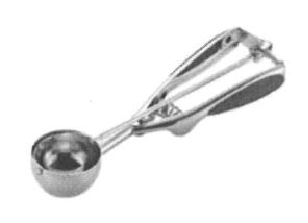
\includegraphics[scale=0.6]{glace}\\
\hspace*{1cm}2 boules: $3,50$ \euro & &\quad Diamètre: $4,2$ cm \rule[-10pt]{0pt}{30pt}\\
\cline{1-1}\cline{3-3} 
\end{tabular}
\end{center}

\begin{center}
{\renewcommand{\arraystretch}{1.2}
\begin{tabularx}{0.5\linewidth}{|*{3}{>{\centering \arraybackslash}X|}}
\multicolumn{3}{c}{\textbf{Nombre de pots de glace vendus\rule[-10pt]{0pt}{0pt}}}\\
\cline{2-3}
\multicolumn{1}{c}{}&\cellcolor{lightgray}Juillet 2022 &\cellcolor{lightgray}Août 2022\\ 
\hline
\cellcolor{lightgray}Semaine 1 & 453 & 860 \\ \hline
\cellcolor{lightgray}Semaine 2 & 649 &\np{1003}\\ \hline
\cellcolor{lightgray}Semaine 3 & 786 & 957 \\ \hline
\cellcolor{lightgray}Semaine 4 & 854 & 838 \\ \hline
\end{tabularx}}
\hfill
\begin{tabular}{|l|}
\hline
\hfill{~}\textbf{Rappels}\hfill{~}\rule[-5pt]{0pt}{20pt}\\
\textbullet~~Le volume d'une boule de rayon $r$\\
\hphantom\textbullet~~est donné par la formule:\\
\hfill{~}$V=\dfrac{4}{3}\times \pi \times r^3$\hfill{~}\rule[-15pt]{0pt}{35pt}\\
\textbullet~~1 dm$^3$ = 1 L\\ \hline
\end{tabular}
\end{center}

\begin{enumerate}
\item Calculer le nombre moyen de pots de glace vendus par semaine au cours de la période de juillet à août 2022.\index{Moyenne}
\item Parmi tous les pots de glace vendus au cours de cette période, 67\,\% sont des pots à une boule. Calculer la somme que rapporte la vente des pots de glace au cours de cette période.\index{Pourcentage}
\item On modélise les boules de glace réalisées avec la cuillère à glace par des boules de $4,2$~cm de diamètre.
	\begin{enumerate}
		\item Montrer que le volume d'une boule de glace est d'environ 39~cm$^3$.\index{Volume boule}
		\item Le vendeur utilise des bacs de glace contenant 10~L chacun.

Combien peut-il faire de boules de glace au maximum, avec la glace contenue dans un bac ?
	\end{enumerate}
\end{enumerate}

\hyperlink{sommaire}{Retour au sommaire}

%%%%%%%%%   fin Asie 19 juin 2023
\newpage
%%%%%%%%%   Polynésie 23 juin 2023

\rfoot{\small{Polynésie}}
\lfoot{\small{23 juin 2023}}
\setlength{\headheight}{13.59999pt}
\marginpar{\rotatebox{90}{\textbf{A. P{}. M. E. P{}.}}}
\pagestyle{fancy}
\thispagestyle{empty}

\phantomsection

\hypertarget{Polynesie}{}
\label{Polynesie}

\begin{center}
{\Large \textbf{\decofourleft~Brevet des collèges Polynésie - 23 juin 2023~\decofourright}}

 \bigskip

\textbf{Durée : 2 heures} \end{center}

\bigskip

\textbf{\large{}Exercice 1 \hfill 16 points}

\medskip

Cet exercice est un questionnaire à choix multiples QCM

\textbf{Aucune justification n'est demandée}

Pour chaque question, trois réponses sont proposées, une seule est exacte.

Écrire sur votre copie, le numéro de la question et la réponse correspondante.

\medskip

\textbf{Question 1 :} soit $f$, la fonction définie par $f(x) = -2x + 3$.

Quelle est la représentation de la fonction $f$ ?\index{Fonction affine}

\medskip

\begin{tabularx}{\linewidth}{*3{>{\centering\arraybackslash}X}}
\textbf{Réponse A}\rule[-7pt]{0pt}{0pt}
\psset{unit=0.4cm}
\def\xmin {-5} \def\xmax {5} \def\ymin {-3} \def\ymax {6}
\begin{pspicture*}(\xmin,\ymin)(\xmax,\ymax)
\psgrid[subgriddiv=1, gridcolor=lightgray]
\psaxes[arrowsize=3pt 2, ticksize=-2pt 2pt,Dx=2,Dy=2,labelFontSize=\scriptstyle]{->}(0,0)(\xmin,\ymin)(\xmax,\ymax)
\psplot[linecolor=blue]{\xmin}{\xmax}{1.5 x mul 3 add}
\end{pspicture*}
&
\textbf{Réponse B}\rule[-7pt]{0pt}{0pt}
\psset{unit=0.4cm}
\def\xmin {-5}   \def\xmax {5} \def\ymin {-3}   \def\ymax {6}
\begin{pspicture*}(\xmin,\ymin)(\xmax,\ymax)
\psgrid[subgriddiv=1, gridcolor=lightgray]
\psaxes[arrowsize=3pt 2, ticksize=-2pt 2pt,Dx=2,Dy=2,labelFontSize=\scriptstyle]{->}(0,0)(\xmin,\ymin)(\xmax,\ymax) 
\psplot[linecolor=blue]{\xmin}{\xmax}{-2 x mul 3 add}
\end{pspicture*}
&
\textbf{Réponse C}\rule[-7pt]{0pt}{0pt}
\psset{unit=0.4cm}
\def\xmin {-5} \def\xmax {5} \def\ymin {-3} \def\ymax {6}
\begin{pspicture*}(\xmin,\ymin)(\xmax,\ymax)
\psgrid[subgriddiv=1, gridcolor=lightgray]
\psaxes[arrowsize=3pt 2, ticksize=-2pt 2pt,Dx=2,Dy=2,labelFontSize=\scriptstyle]{->}(0,0)(\xmin,\ymin)(\xmax,\ymax) 
\psplot[linecolor=blue]{\xmin}{\xmax}{3 x mul 2 sub}
\end{pspicture*}
\end{tabularx}

\medskip

\begin{minipage}{0.65\linewidth}\textbf{Question 2 :}
On considère la fonction dont la représentation graphique est donnée ci-contre.

D'après le graphique, quelle est l'image de 1 par cette fonction ?

\begin{tabularx}{\linewidth}{*{2}{>{\centering \arraybackslash}X|}{>{\centering \arraybackslash}X}}
Réponse A  &Réponse B&  Réponse C\\ 
L’image de 1 est 2&L’image de 1 est $-2$&L’image de 1 est 0\\
\end{tabularx}
\end{minipage}\hfill
\begin{minipage}{0.28\linewidth}
\psset{unit=0.6cm}
\def\xmin {-3} \def\xmax {3} \def\ymin {-3}   \def\ymax {3}
\begin{pspicture*}(\xmin,\ymin)(\xmax,\ymax)
\psgrid[subgriddiv=1, gridcolor=lightgray]
\psaxes[arrowsize=3pt 2, ticksize=-2pt 2pt,Dx=2,Dy=2,labelFontSize=\scriptstyle]{->}(0,0)(\xmin,\ymin)(\xmax,\ymax) 
\psplot[linecolor=blue]{\xmin}{\xmax}{-5 x dup mul mul 17 add x mul 6 div}
\psdots[linecolor=blue](-2,1)(-1,-2)(1,2)(2,-1)
\uput[dl](-2,1){\blue A} \uput[dl](-1,-2){\blue B} 
\uput[ur](1,2){\blue C} \uput[ur](2,-1){\blue D} 
\end{pspicture*}
\end{minipage}

\medskip

\textbf{Question 3 :}

On donne ci-dessous un tableau de valeurs de la fonction $h$ définie par $h(x) = - x + 1$ réalisé à l'aide d'un tableur :

\begin{center}
$\begin{array}{|>{\cellcolor{lightgray}}c| *{7}{>{\centering\arraybackslash}m{1cm}|}}
\cline{2-8}
\rowcolor{lightgray} &\text A & \text B & \text C & \text D & \text E & \text F & \text G\\
\hline
1 & \blue $x$ & -3 & -2 & -1 & 0 & 1 & 2 \\ \hline
2 & \blue $h(x)$  & 4 & 3 & 2 & 1 & 0 & -1 \\ \hline
\end{array}$
\end{center}

Quelle formule a-t-on saisie dans la case B2 avant de l'étirer vers la droite ?\index{Tableur}

\begin{tabularx}{\linewidth}{*{2}{>{\centering \arraybackslash}X|}{>{\centering \arraybackslash}X}}
Réponse A  &Réponse B&  Réponse C\\ 
= $- (-3) + 1$ &= $- x + 1$ & = $-$ B1 + 1\\
\end{tabularx}

\medskip

\textbf{Question 4 :}

Quelle est la forme développée de l'expression $(3x - 7)^2$ ?\index{Calcul littéral}

\begin{tabularx}{\linewidth}{*{2}{>{\centering \arraybackslash}X|}{>{\centering \arraybackslash}X}}
Réponse A	&Réponse B			&Réponse C\\ 
$3x^2 - 49$	& $9x^2 - 42x + 49$	&$9x^2 - 49$.
\end{tabularx}

\newpage

\textbf{\large{}Exercice 2 \hfill 16 points}

\medskip

Olivia a décidé d'installer sur le sol, plat de son jardin, quatre panneaux photovoltaïques pour produire une partie de l'électricité qu'elle consomme.

\medskip

\begin{tabularx}{\linewidth}{|X|}\hline
\textbf{Description}\\
Un panneau photovoltaïque est un dispositif permettant de générer de l'électricité à partir de l'énergie lumineuse.\\
\textbf{Caractéristiques d'un panneau}

\begin{itemize}
\item[$\bullet~~$] Longueur 1700 mm
\item[$\bullet~~$] Largeur 1000 mm
\item[$\bullet~~$] Épaisseur 40 mm
\item[$\bullet~~$] Fonctionnement optimal : inclinaison par rapport à l’horizontale comprise entre $30\degres$ et $35\degres$
\item[$\bullet~~$] Orientation : Sud
\end{itemize}\\ \hline
\end{tabularx}

\smallskip

Pour incliner ses panneaux et obtenir un fonctionnement optimal, Olivia choisit de fabriquer elle-même un support. Pour cela, elle réalise les schémas suivants de support qui sera constitué de trois équerres identiques, reliées entre elles par trois barres latérales de $4$~m de long.
Chaque support est prévu pour accueillir quatre panneaux.

\medskip

\begin{tabularx}{\linewidth}{p{7cm}|X}
Plan général du support, un panneau est représenté : &Plan détaillé d’une équerre :\\
\psset{unit=0.8cm,arrowsize=2pt 3}
\begin{pspicture}(8.2,4.4)
%\psgrid
\pspolygon[linewidth=0.8pt](0,2.8)(0,1.1)(2.2,1.1)(8.2,2.6)(6,4.3)
\psline[linestyle=dotted,linewidth=1.25pt](0,1.1)(6,2.6)
\pspolygon[linestyle=dotted,linewidth=1.25pt](3,3.52)(3,1.82)(5.2,1.82)
\pspolygon[linestyle=dotted,linewidth=1.25pt](6,4.3)(6,2.6)(8.2,2.6)
\psline[linestyle=dotted,linewidth=1.25pt](0.9,1.1)(0.9,2.1)
\psline[linestyle=dotted,linewidth=1.25pt](3.8,1.9)(3.8,2.8)
\psline[linestyle=dotted,linewidth=1.25pt](6.8,2.7)(6.8,3.6)
\pspolygon[fillstyle=solid,fillcolor=lightgray](0,2.8)(1.5,3.15)(3.7,1.45)(2.2,1.1)
\rput(6,0.1){Barres latérales}
\psline{->}(6,0.2)(7,2.3)
\psline{->}(6,0.2)(4.8,4)
\psline{->}(6,0.2)(0.6,1.22)
\psline{<->}(0,2.9)(6,4.4)\uput[u](3,3.65){4~m}
\end{pspicture}&
\psset{unit=0.9cm,arrowsize=2pt 3}
\begin{pspicture}(6.8,4.4)
\pspolygon[linewidth=1.4pt](1.1,0.8)(6.6,0.8)(1.1,3.9)
\psline[linewidth=1.4pt](2.2,0.8)(2.2,3.3)
\psframe(1.1,0.8)(1.3,1)\psframe(2.2,0.8)(2.4,1)
\uput[ul](1.1,3.9){H} \uput[l](1.1,0.8){P} \uput[ur](2.2,3.3){U} \uput[ul](2.2,0.8){T} \uput[r](6.6,0.8){S}
\psline[linewidth=0.65pt]{<->}(1.1,0.6)(6.6,0.6)\uput[d](3.85,0.6){140~cm}
\rput{90}(0.9,2.35){90~cm}
\end{pspicture}
\end{tabularx}
\medskip

\begin{enumerate}
\item 
	\begin{enumerate}
		\item Vérifier que la distance HS arrondie au millimètre est égale à 166,4 cm.\index{Pythagore}
		\item Pour que le panneau soit bien tenu, le fabricant conseille que la distance HS du support mesure au moins 95\,\% de la longueur du panneau.
		
On rappelle que cette longueur mesure \np{1700}~mm.

Ce support sera-t-il conforme aux conseils du fabricant ?\index{Pourcentage}
	\end{enumerate}
\item L’angle d’inclinaison, $\widehat{\text{HSP}}$ permettra-t-il un fonctionnement optimal des panneaux ?
\item Pour consolider l’ensemble, Olivia fixe, à l’intérieur de ses équerres, une barre de renfort de $50$~cm de longueur.

Sur le plan détaillé d’une équerre, cette barre est représentée par le segment [UT] perpendiculaire au segment [PS].

Calculer la longueur ST. On arrondira au millimètre.\index{Thalès}
\item Olivia, achète des tubes en acier inoxydable de longueur $4,5$~m à $37$~\euro{} l’unité pour fabriquer le support composé de trois équerres et des trois barres latérales.
Montrer qu’elle doit prévoir un budget minimum de $222$~\euro{} pour l’achat des tubes en acier inoxydable.
\end{enumerate}

\bigskip

\textbf{\large{}Exercice 3 \hfill 18 points}

\medskip

Dans cette exercice, on étudie la probabilité de gain des deux jeux ci-dessous.

\bigskip

\textbf{Partie A }

\medskip

\begin{tabularx}{\linewidth}{X|X}
Jeu 1&Jeu 2\\
Un sac contient cinq boules indiscernables au toucher, dont une portant la lettre N, deux, portant la lettre G et deux portant la lettre P.& Une roue à six  secteurs angulaires identiques numérotées de un à six.\\
\qquad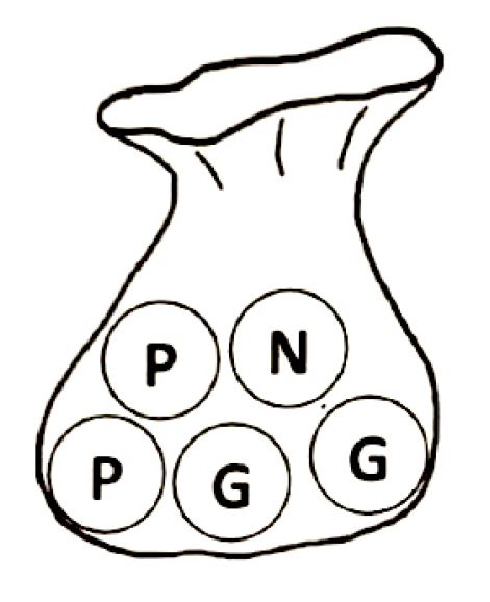
\includegraphics[scale=0.5]{Jeu1}&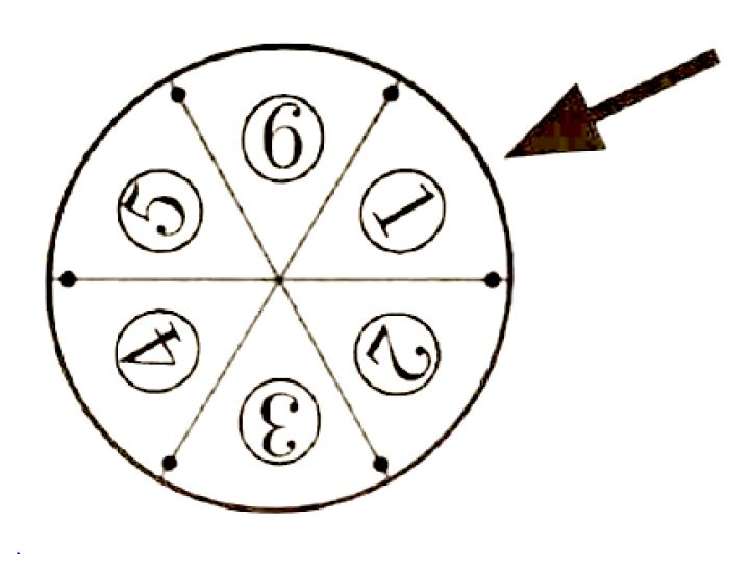
\includegraphics[scale=0.5]{Jeu2}
\end{tabularx}

\medskip

\begin{enumerate}
\item On considère le jeu 1.

On pioche une boule au hasard dans ce sac et on note la lettre inscrite sur la boule choisie.

On considère qu'on a gagné si on pioche la lettre G.

Montrer que la probabilité de gagner avec ce jeu et de $\dfrac25$.
\item On considère le jeu 2.

On fait tourner la roue et on note le nombre d'inscrits sur le secteur pointé par la flèche. 

On considère qu'on a gagné si on s'arrête sur un nombre premier.

Quelle est la probabilité de gagner à ce jeu ?\index{Probabilité}
\item 
	\begin{enumerate}
		\item Quel est le jeu qui présente la plus faible probabilité de gagner ?
		\item Proposer une liste de boules à rajouter pour que la probabilité de gagner avec le jeu 1 soit de $\dfrac14$.
	\end{enumerate}
\end{enumerate}

\bigskip

\textbf{Partie B}

\medskip

\textbf{Dans cette partie, toute trace de recherche sera valorisée.}

\medskip

On choisit finalement de combiner ces deux jeux.

Dans un premier temps, le joueur doit tirer une boule dans le sac du jeu 1.

On doit ensuite faire tourner la roue du jeu 2.

Le joueur gagne un lot s'il a tiré une boule portant la lettre G et si la roue s'arrête sur un secteur angulaire dont le numéro est un nombre premier.

Quelle est la probabilité de gagner à cette combinaison des deux jeux ?

\newpage

\textbf{\large{}Exercice 4 \hfill 22 points}

\medskip

On considère le programme de calcul suivant :

\medskip

\begin{itemize}
\item[$\bullet~~$]Choisir un nombre
\item[$\bullet~~$]Prendre le carré de ce nombre
\item[$\bullet~~$]Multiplier le résultat par 2
\item[$\bullet~~$]Ajouter le nombre de départ
\item[$\bullet~~$]Soustraire 66
\end{itemize}

\medskip

\begin{enumerate}
\item 
	\begin{enumerate}
		\item Montrer que si le nombre choisi au départ est 4, le résultat obtenu est $-30$.\index{Calcul numérique}
		\item  Quel résultat obtient-on si le nombre choisi au départ est $-3$ ?
	\end{enumerate}
\item 
	\begin{enumerate}
		\item On s'intéresse au bloc d'instruction ci-dessous intitulé \og Programme de calcul \fg.
On souhaite le compléter pour calculer le résultat obtenu avec le programme de calcul en fonction du nombre choisi au départ.

On précise que deux variables ont été créées: \og nombre choisi\fg{} qui correspond au nombre choisi au départ, et \og Résultat \fg.\index{Scratch}

\begin{center}
\begin{scratch}
\initmoreblocks{définir \namemoreblocks{Programme de calcul}}
\blockvariable{mettre \selectmenu{Résultat} à \ovaloperator{\ovalnum{A} * \ovalvariable{Nombre choisi}}}
\blockvariable{mettre \selectmenu{Résultat} à \ovaloperator{\ovalnum{B} * \ovalvariable{Résultat}}}
\blockvariable{mettre \selectmenu{Résultat} à \ovaloperator{\ovalvariable{Résultat} + \ovalvariable{Nombre choisi}}}
\blockvariable{mettre \selectmenu{Résultat} à \ovaloperator{\ovalvariable{Résultat} - \ovalnum{66}}}
\end{scratch}
\end{center}

Écrire sur votre copie le contenu qui doit être inséré dans les emplacements A et B. 
\textbf{Aucune justification n'est attendue pour cette question.}

		\item  Lucie insère le bloc précédent dans le script ci-dessous et observe la réponse donnée par le lutin:

\medskip

\begin{minipage}{0.6\linewidth}
\begin{center}
Script
\end{center}
\begin{scratch}
\blockinit{Quand \greenflag est cliqué}
\blockvariable{mettre \selectmenu{nombre choisi} à \ovalnum{0}}
\blockrepeat{répéter \ovalnum{20} fois}
{
\blocklist{Programme de calcul}
\blockif{si \booloperator{\ovalmove{Résultat} = \ovalnum{0}} alors}
{
\blocksound{dire \ovaloperator{regrouper \ovalnum{On peut choisir comme nombre de départ} et}\ovalvariable{nombre choisi}} 
}
\blockvariable{mettre \selectmenu{nombre choisi} à \ovaloperator{\ovalvariable{nombre choisi} + \ovalnum{0,5}}}
}
\end{scratch}
\end{minipage}
\begin{minipage}{0.37\linewidth}
\begin{center}
Réponse du lutin\\
\end{center}
On peut choisir comme nombre de départ $5,5$.\\
\\
\qquad
\includegraphics[scale=0.7]{Lutin}\\
\\
\\
\\
\\
\\
\\
\\
\\
\\
\end{minipage}

\medskip

À quoi correspond la valeur 5,5 donnée comme réponse par le lutin avec le programme de Lucie?
	\end{enumerate}
\item On nomme $x$ le nombre choisi au départ.
	\begin{enumerate}
		\item Déterminer l'expression obtenue par ce programme de calcul en fonction de $x$.
		\item On admet que $(2x - 11) (x + 6)$ est la forme factorisée de l'expression trouvée à la question précédente.
		
Pour quelle(s) valeur(s) de $x$, le résultat obtenu avec le programme est-il égal à $0$ ?\index{Equation-produit@Équation-produit}
	\end{enumerate}
\end{enumerate}

\bigskip

\textbf{\large{}Exercice 5 \hfill 22 points}

\medskip

Un professionnel et un amateur vont faire une séance de karting sur la piste ci-dessous (représentée en traits pleins).

Cette piste est constituée de segments, de demi-cercles et de quarts de cercles.

Le professionnel fait un tour de piste en $60$ secondes.

L'amateur fait un tour de piste en $72$ secondes.


\begin{center}
\psset{unit=0.9cm}
\begin{pspicture}(16.4,11.6)
%\psgrid
\psset{linewidth=1.3pt}
\psline(3,0.6)(8.4,0.6)%CB
\psline(9.8,2)(9.8,4.5)%AL
\psline(11,5.9)(13.7,5.9)%KJ
\psline(13.7,11.2)(9.6,11.2)%IH
\psline(8.2,10)(8.2,7.3)%GF
\psline(3,6)(7,6)%ED
\psarc(8.4,2){1.4}{-90}{0}
\psarc(11.2,4.5){1.4}{90}{180}
\psarc(13.7,8.55){2.65}{-90}{90}
\psarc(9.6,9.8){1.4}{90}{180}
\psarc(6.8,7.4){1.4}{-90}{0}
\psarc(3,3.3){2.7}{90}{270}
\psset{linewidth=1pt}
\psline[linestyle=dashed](3,0.6)(3,6)%CD
\psline[linestyle=dashed](0.25,3.3)(3,3.3)
\psline[linestyle=dashed](8.4,0.6)(8.4,2)(9.8,2)%BXA
\psline[linestyle=dashed](9.8,4.5)(11,4.5)(11,5.9)%JXL
\psline[linestyle=dashed](13.7,5.9)(13.7,11.2)%JI
\psline[linestyle=dashed](13.7,8.55)(16.4,8.55)
\psline[linestyle=dashed](9.6,11.2)(9.6,9.8)(8.2,9.8)%HXG
\psline[linestyle=dashed](8.2,7.3)(7,7.3)(7,6)%FXE
\psframe(3,3.3)(2.8,3.5)\psframe(7,7.3)(7.2,7.1)
\psframe(13.7,8.55)(13.9,8.35) \psframe(11,4.5)(10.8,4.7)
\psframe(8.4,2)(8.6,1.8)
\uput[r](9.8,2){A} \uput[d](8.4,0.6){B} \uput[d](3,0.6){C} \uput[u](3,6){D \small (Départ)} 
\uput[d](7,6){E} \uput[r](8.2,7.3){F} \uput[l](8.2,10){G} \uput[u](9.6,11.2){H} 
\uput[u](13.7,11.2){I} \uput[d](13.7,5.9){J}  \uput[u](11,5.9){K} \uput[l](9.8,4.5){L}
\psline(6.9,6.55)(7.1,6.55)\psline(7.6,7.2)(7.6,7.4)
\psline(8.3,1.3)(8.5,1.3)\psline(9.1,1.9)(9.1,2.1)
\psline(10.4,4.4)(10.4,4.6)\psline(10.9,5.2)(11.1,5.2)
\psline(8.9,9.7)(8.9,9.9)\psline(9.5,10.5)(9.7,10.5)
\psdots[dotstyle=+,dotangle=45,dotscale=2.2](14.9,8.55)(13.7,7.2)(13.7,9.9)(1.5,3.3)(3,1.8)(3,4.6)(8.2,8.5)(12.4,5.9)(9.8,3.25)
\psdots[dotstyle=square*,dotscale=1.5](5,6)(11.85,11.2)% 90 m
\uput[u](5,6){90~m}\uput[d](5.7,0.6){120~m}\uput[r](9.8,3.25){60~m}
\uput[r](9.6,10.6){30~m}
\end{pspicture}
\end{center}

\begin{enumerate}
\item Montrer que la longueur de la piste est de \np{1045}~m, arrondie à l'unité près.\index{Longueur du cercle}

Toute trace de recherche sera valorisée.
\item Calculer la vitesse moyenne du professionnel en m/s. On arrondira au centième près.\index{Vitesse}
\item Pour des raisons de sécurité sur ce circuit, les amateurs ne doivent pas dépasser les $60$~km/h de moyenne. Cet amateur respecte-t-il les règles de sécurité ?
\item Le professionnel et l'amateur partent en même temps de la ligne de départ et font plusieurs tours de circuit.

On rappelle que le professionnel effectue un tour en $60$~s et l'amateur en $72$~s.
	\begin{enumerate}
		\item Décomposer $60$ et $72$ en produit de facteurs premiers.\index{Produit de facteurs premiers}
		\item Au bout de combien de temps se retrouveront-ils pour la première fois sur la ligne de départ ensemble ?\index{Plus petit multiple commun}
		\item Combien auront-ils alors effectué de tours chacun ?
	\end{enumerate}
\end{enumerate}

\hyperlink{sommaire}{Retour au sommaire}
%%%%%%%%%   fin Polynésie 23 juin 2023
\newpage
%%%%%%%%%   Métropole Antilles--Guyane 26 juin 2023

\rfoot{\small Métropole  Antilles-Guyane }
\lfoot{\small 26 juin 2023}
\pagestyle{fancy}
\thispagestyle{empty}

\phantomsection

\hypertarget{Metropole}{}
\label{Metropole}

\begin{center} {\Large \textbf{\decofourleft~Brevet Métropole Antilles-Guyane - 26 juin 2023 \decofourright}}
\end{center}

\bigskip

{\large \textbf{Exercice 1 \hfill 20 points}}

\medskip

Un opticien vend différents modèles de lunettes de soleil.

Il reporte dans le tableur ci-dessous des informations sur cinq modèles vendus pendant l'année 2022.

\begin{center}
	\begin{tabularx}{\linewidth}{|c|>{\centering \arraybackslash}m{4cm}|*{6}{>{\centering \arraybackslash}X|}} \hline
	 & \textsf{A} & \textsf{B} & \textsf{C} & \textsf{D} & \textsf{E} & \textsf{F} & \textsf{G}\\ \hline
 	\textsf{1} & \textbf{Lunettes de soleil} & \textbf{Modèle 1} & \textbf{Modèle 2} & \textbf{Modèle 3} & \textbf{Modèle 4} & \textbf{Modèle 5} & \textbf{Total}\\ \hline
	\textsf{2} & \textbf{Nombre de paires de lunettes vendues} & \np{1200} & 950 & 875 & 250 & 300 & \\ \hline
	\textsf{3} & \textbf{Prix à l'unité en euro} & 75 & 100 & 110 & 140 & 160 & \\ \hline
\end{tabularx}
\end{center}

\begin{enumerate}
	\item Montrer que l'étendue des prix de ces paires de lunettes de soleil est de 85 euros.\index{Etendue@Étendue}

	\item \begin{enumerate}
		\item Quelle formule doit-on saisir dans la cellule G2 pour calculer le nombre total de paires de lunettes de soleil vendues en 2022 ?\index{Tableur}
		\item Calculer le nombre total de paires de lunettes de soleil vendues en 2022.
	\end{enumerate}
	\item \begin{enumerate}
		\item Calculer le montant total, en euros, des ventes des paires de lunettes de soleil en 2022.
		\item Calculer le prix moyen d'une paire de lunettes de soleil vendue en 2022 , arrondi au centime près.\index{Moyenne}
	\end{enumerate}
\end{enumerate}

\vspace{5mm}

%%%%%%%%
{\large \textbf{Exercice 2 \hfill20 points}}

\bigskip

Sur la figure ci-dessous :

\begin{itemize}[label={\textbullet~}]
	\item BCDE est un rectangle, BAE est un triangle rectangle en A ;
	\item la perpendiculaire à la droite (CD) passant par A coupe cette droite en H;
	\item les droites (AE) et (CD) se coupent en F.
\end{itemize}
\begin{center}
	\begin{tikzpicture}[x=7mm,y=7mm]
	\draw[line width=1pt] (0,0) node[below left]{C}--
		(12.6,0.) node[below right] {F}--
		(2.52,7.56) node[pos = 0.28, sloped]{|||} node[above]{A}--
		(0.,4.2)node[pos = 0.5, sloped]{||} node[above left]{B} --cycle node[pos = 0.5, sloped]{||}
		(0.,4.2) -- (7.,4.2)node[pos = 0.5, sloped]{|||} node[above right]{E} -- (7.,0.) node[below right]{D}
		(2.52,0.) node[below] {H} -- (2.52,7.56);
		\foreach \x/\y in {0/0 , 2.52/0, 6.6/0, 6.6/3.8, 0/3.8}
			\draw[shift={(\x,\y)}] (0,0) rectangle (0.4,0.4) ;
		\draw[shift={(2.52,7.56)},rotate=143.13] (0,0) rectangle (-0.4,0.4) ;
\end{tikzpicture}
\end{center}

\newpage

On donne :
\begin{itemize}[label={\textbullet~}]
	\item $\mathrm{AB}=\mathrm{BC}=4,2 \mathrm{~cm}$;
	\item $\mathrm{EB}=\mathrm{EF}=7 \mathrm{~cm}$.
\end{itemize}

\begin{enumerate}
\item Montrer que l'aire du rectangle BCDE est égale à \np[cm^2]{29,4}.
\item 
	\begin{enumerate}
		\item Montrer que la longueur AE est égale à \np[cm]{5,6}.\index{Pythagore}
		\item Calculer l'aire du triangle rectangle ABE.\index{Aire du triangle}
	\end{enumerate}
\item 
	\begin{enumerate}
		\item Montrer que les droites (ED) et (HA) sont parallèles.\index{Droites parallèles}
		\item Calculer la longueur AH.
	\end{enumerate}
\end{enumerate}

\vspace{5mm}

{\large \textbf{Exercice 3 \hfill20 points}}

\medskip

Cet exercice est un questionnaire à choix multiple (QCM).

Pour chaque question, trois réponses (A, B ou C) sont proposées.

\textbf{Une seule réponse est exacte.}

\textbf{Recopier sur la copie} le numéro de la question et la réponse choisie. Aucune justification n'est demandée.

\medskip

\begin{tabularx}{\linewidth}{|m{7cm}|*{3}{>{\centering \arraybackslash}X|}} \hline
	\centering\textbf{Question}& \textbf{Réponse A}& \textbf{Réponse B}& \textbf{Réponse C}\\ \hline
\textbf{1.} Dans une classe de 25 élèves, $60 \%$ des élèves sont des filles.

Combien y a-t-il de filles dans cette classe ?\index{Pourcentage}
	& 10 & 15 & 20 \\ \hline

\textbf{2.} Quelle est la décomposition en produit de facteurs premiers de 126 ?\index{Produit de facteurs premiers}
	& $2 \times 9 \times 7$ & $2^2 \times 5^2 + 2 \times 13$ &$2 \times 3^2 \times 7$ \\ \hline

\textbf{3.} Dans un sac, il y a 17 jetons rouges, 23 jetons jaunes et 20 jetons bleus, tous indiscernables au toucher. On tire au hasard un jeton du sac.

Quelle est la probabilité d'obtenir un jeton rouge ou un jeton jaune ?\index{Probabilité}
	&$\dfrac{2}{3}$ & 0,6 & $\dfrac{17}{23}$  \\ \hline

\textbf{4.} Sur l'octogone régulier ci-dessous, quelle est l'image du segment [DC] par la rotation de centre O qui transforme A en D?\index{Rotation}

	\hfill~	\begin{tikzpicture}[]
		\foreach \a/\n in {1/A, 2/B, 3/C, 4/D, 5/E, 6/F, 7/G, 8/H}
			\draw (0,0)--(-100+45*\a:1.5) node[shift={(-100+45*\a:0.3)}]{\n}--(-55+45*\a:1.5);
		\node at (-0.1,-0.2){O};
	\end{tikzpicture}\hfill~
	& [GE] & [GF] & [AH]\\ \hline

\textbf{5.} Quel est le volume d'un pavé droit de hauteur \np[m]{1,5} et de base rectangulaire de \np[m]{2} de longueur et \np[m]{1,3} de largeur ?\index{Volume du pavé}

{\small \emph{On rappelle que $\np[m^3]{1}=\np[L]{1000}$.}}
	&\np[m^3]{2,6} & \np[L]{3900}& \np[L]{3000} \\ \hline
\end{tabularx}

\newpage

%%%%%%%%
{\large \textbf{Exercice 4 \hfill 20 points}}

\bigskip

On veut fabriquer un escalier en bois de hauteur \np[cm]{272}.

La figure ci-dessous représente une vue de profil de cet escalier.

La hauteur d'une marche est de \np[cm]{17}.

La profondeur d'une marche pour poser le pied mesure \np[cm]{27}.

\begin{center}
\begin{tikzpicture}[line cap = round,>=stealth,x =8mm]
   \draw[dashed] (0,0)--(-1,0) (0,0.8)--(-1,0.8) ;
   \draw[<->] (-1,0)--(-1,0.8) node[pos=0.5,left, text width=2cm,align=center]{Hauteur d'une marche} ;
   \draw[dashed] (0,0.8)--(0,3) (1.6,0.8)--(1.6,3) ;
\draw[<->] (0,3)--(1.6,3) node[pos=0.5,above, text width=2cm,align=center]{Profondeur d'une marche} ;
   \draw[dashed] (10.8,0)--(11.8,0) (10.8,5.4)--(11.8,5.4) ;
   \draw[<->] (11.8,0)--(11.8,5.4) node[pos=0.5,right, text width=2cm,align=center]{Hauteur de l'escalier} ;
   \draw (4.8,2.4)--(0,0)node[below left]{A}--(10.8,0)node[below right]{B}--(10.8,5.4)node[above right]{C}--(9.2,4.6) ;
   \draw[dotted] (4.8,2.4)--(9.2,4.6) ;
   \draw[line width=1pt] (0,0)--(0,0.8)--(1.6,0.8)--
   (1.6,1.6)--(3.2,1.6)--(3.2,2.4)--(4.8,2.4)
   (9.2,4.6)--(9.2,5.4)--(10.8,5.4);
   \draw[dotted, line width=1pt] (4.8,2.4)--(4.8,3.2)--(6.4,3.2)
   (9.2,4.6)--(7.6,4.6)--(7.6,3.8);
   \draw (10.8,0) rectangle ++(-4mm,4mm);
\end{tikzpicture}
\end{center}

\begin{enumerate}
	\item \begin{enumerate}
		\item Montrer qu'il faut prévoir 16 marches pour construire cet escalier.
		\item Montrer que la longueur AB est égale à \np[cm]{432}.
	\end{enumerate}
	\item Pour permettre une montée agréable, l'angle $\widehat{\mathrm{BAC}}$ doit être compris entre $25^{\circ}$ et $40^{\circ}$.
	\begin{enumerate}
		\item Calculer la mesure de l'angle $\widehat{\mathrm{BAC}}$, arrondie au degré près.\index{Trigonométrie}
		\item L'escalier permet-il une montée agréable ?
	\end{enumerate}
	\item \begin{minipage}[t]{7.5cm}
		On rédige le programme ci-contre avec le logiciel Scratch pour dessiner cet escalier.
	(\np[cm]{1} dans la réalité est représenté par 1 pas dans le programme.)

	\textbf{Recopier} les lignes $5,6,7$ et 9 \textbf{sur la copie} en les complétant.\index{Scratch}
	\end{minipage}\hfill
	\begin{scratch}[num blocks]
		\blockinit{Quand \greenflag{} est cliqué}
		\blockmove{s'orienter à \ovalnum{90}}
		\blockpen{effacer tout}
		\blockpen{stylo en position d'écriture}
		\blockrepeat{répéter \ovalnum{\dots} fois}{
		\blockmove{tourner \turnleft{} de \ovalnum{\dots} degrés}
		\blockmove{avancer de \ovalnum{\dots} pas}
		\blockmove{tourner \turnright{} de \ovalnum{90} degrés}
		\blockmove{avancer de \ovalnum{\dots} pas}}
	\end{scratch}
\end{enumerate}

\newpage

\textbf{Exercice 5 \hfill 20 points}

\medskip

Voici deux programmes de calcul.

\begin{center}
	\begin{tabularx}{\linewidth}{|X|X|}\hline
Programme A &Programme B\\
$\bullet~~$ Choisir un nombre				&$\bullet~~$ Choisir un nombre\\
$\bullet~~$ Multiplier ce nombre par $-2$	&$\bullet~~$ Soustraire 5 à ce nombre\\
$\bullet~~$ Ajouter 5 à ce résultat.		&$\bullet~~$ Multiplier le résultat par 3\\
											&$\bullet~~$ Ajouter 11 au résultat\\ \hline
	\end{tabularx}
\end{center}

\begin{enumerate}
\item
	\begin{enumerate}
		\item Montrer que, si on choisit $- 3$ comme nombre de départ, le résultat obtenu avec le programme A est 11.
		\item Quel résultat obtient-on avec le programme B si on choisit 5,5 comme nombre de départ ?
	\end{enumerate}
\item En désignant par $x$ le nombre de départ, on obtient $- 2x + 5$ comme résultat avec le programme A.

	Montrer, qu'avec le même nombre de départ, le résultat du programme B est égal à $3x - 4$.
\end{enumerate}
\begin{minipage}{0.56\linewidth}
	\begin{enumerate}[resume]
		\item
		\begin{enumerate}
			\item On a représenté ci-contre les fonctions $f$ et $g$ définies par $f(x) = -2x + 5$ 
et $g(x) = 3x - 4$.

Associer, en justifiant, chaque droite à la fonction qui lui correspond.
			\item Par lecture graphique, donner, le plus précisément possible, le nombre dont l'image est la même par la fonction $f$ et la fonction $g$.\index{Fonction affine}
		\end{enumerate}
	\end{enumerate}
\end{minipage}\hfill
\begin{minipage}{0.42\linewidth}
	\psset{xunit=1cm,yunit=0.7cm,arrowsize=2pt 3}
	\begin{pspicture*}(-1.02,-5)(5,7.02)
		\psgrid[gridlabels=0pt,subgriddiv=1,gridcolor=lightgray]
		\psaxes[linewidth=1.25pt,labelFontSize=\scriptstyle]{->}(0,0)(-0.99,-4.99)(5,7)
		\psplot[plotpoints=500,linewidth=1.25pt,linecolor=blue]{-1}{5}{x 3 mul 4 sub}\uput[dr](3,5){\blue $(D_1)$}
		\psplot[plotpoints=500,linewidth=1.25pt,linecolor=blue]{-1}{5}{5 x 2 mul sub}\uput[ur](4,-3){\blue $(D_2)$}
	\end{pspicture*}
\end{minipage}

\medskip

\begin{enumerate}[start=4]
	\item Déterminer par le calcul le nombre de départ pour lequel les programmes A et B donnent le même résultat.\index{Calcul numérique}
\end{enumerate}

\hyperlink{sommaire}{Retour au sommaire}
%%%%%%%%   fin Métropole 26 juin 2023
\newpage
%%%%%%%%%   Polynésie septembre 2023
\hypertarget{Polynesiesep}{}
\label{Polynesiesep}

\rfoot{\small Polynésie}
\lfoot{\small 11 septembre 2023}
\pagestyle{fancy}
\thispagestyle{empty}
\begin{center}
{\Large\textbf{\decofourleft~ Diplôme national du Brevet Polynésie
 ~\decofourright}}\\[7pt]
{\Large \textbf{11 septembre 2023}}

\vspace{0,5cm}

\textbf{Durée : 2 heures}
\end{center}
\medskip

\textbf{{\large \textsc{Exercice 1}} \hfill 16 points}

\medskip

Cet exercice est un questionnaire à choix multiples (QCM).\index{QCM}

Pour chaque question, parmi les réponses proposées, une seule est exacte.

Recopier le numéro de la question et indiquer la réponse choisie avec la justification.

\medskip

\begin{center}
\begin{tabularx}{\linewidth}{|m{7.5cm}|*{3}{>{\centering \arraybackslash}X|}}\hline
\multicolumn{1}{|c|}{Questions}&Réponse A&Réponse B&Réponse C\\ \hline
\textbf{1.~} Une augmentation de 9\,\% correspond à une multiplication par \ldots&1,9&$\dfrac{9}{100}$&1,09\\ \hline\index{Pourcentage}
\textbf{2.~} On considère la figure ci-dessous:

\psset{unit=1cm}
\begin{pspicture}(-1.8,-0.4)(5,2.5)
\pspolygon(0,0)(3.7;0)(4.7;25)%ABC
\psline(1.1;0)(1.3973;25)%DE
\uput[dl](0,0){A} \uput[dr](3.7;0){B} \uput[ur](4.7;25){C} \uput[d](1.1;0){D} \uput[u](1.3973;25){E} 
\end{pspicture}

On précise que :

\begin{itemize}
\item[$\bullet~$] (DE) et (BC) sont parallèles;
\item[$\bullet~$] E est un point de [AC];
\item[$\bullet~$] D est un point de [AB];
\item[$\bullet~$] AE = 2~cm, EC = 5~cm, ED = 3~cm.
\end{itemize}\index{Thalès}

Quelle est la longueur BC ?&7,5~cm&6~cm&10,5~cm\\ \hline
\textbf{3.~} Le tableau ci-dessous donne la répartition des élèves de 5\up{e} d'un collège en fonction du sexe et de la langue vivante 2 choisie :

\begin{tabular}{|l|*{3}{c|}}\hline
\multicolumn{1}{|l|}{~}	&Allemand 	& Espagnol 	& Italien\\ \hline
Filles 					&10 		&43 		&26 \\ \hline
Garçons					&7			&42			&32\\ \hline
\end{tabular}

On interroge au hasard un élève de 5\up{e} parmi tous les élèves de 5\up{e} de ce collège.

Quelle est la probabilité que l'élève interrogé ait choisi l'italien en deuxième langue vivante ?
\index{Probabilité}
&$\dfrac{1}{3}$	&$\dfrac{58}{160}$	&$\dfrac{58}{102}$\\ \hline
\textbf{4.~} On reprend la situation de la question \textbf{3.~} et on interroge au hasard un élève de 5\up{e} parmi tous les élèves de 5\up{e} de ce collège.

Quelle est la probabilité que l'élève interrogé soit une fille qui ne fait pas d'allemand ?
&$\dfrac{69}{79}$	&$\dfrac{69}{143}$	&$\dfrac{69}{160}$\\ \hline
\end{tabularx}
\end{center}

\newpage

\textbf{{\large \textsc{Exercice 2}} \hfill 25 points}

\medskip

\begin{minipage}{7.4cm}
\begin{enumerate}
\item On considère le programme A défini par le schéma ci-contre :\index{Programme de calcul}
	\begin{enumerate}
		\item Vérifier que le résultat est $60$ si le nombre
choisi au départ est $-8$.
		\item On appelle $x$ le nombre de départ et on admet que le résultat obtenu avec le programme de calcul est donné par l'expression :

$(x + 3)(x - 4)$.

Résoudre $(x + 3)(x - 4) = 0$.

En déduire quels nombres de départ il faut choisir pour obtenir 0 comme résultat.
	\end{enumerate}
\end{enumerate}
\end{minipage}\hfill
\begin{minipage}{7.5cm}
\psset{unit=1cm,arrowsize=2pt 3}
\begin{pspicture}(-3.8,0)(3.8,7.4)
%\psgrid
\psframe(-0.9,5.4)(0.9,6.2)\psframe(-0.9,0)(0.9,0.8)
\psframe(-3.8,3.1)(-2,3.9)\psframe(3.8,3.1)(2,3.9)
\rput(-2.3,4.8){Ajouter 3}\rput(2.7,4.8){Soustraire 4}
\rput(0,7.1){Choisir un nombre}
\rput(0,2.7){Multiplier les deux}\rput(0,2.2){résultats}
\psline{->}(0,6.9)(0,6.2)\psline{->}(0,5.4)(-2.9,3.9)\psline{->}(0,5.4)(2.9,3.9)
\psline(-2.9,3.1)(0,1.4)\psline(2.9,3.1)(0,1.4)
\psline{->}(0,1.4)(0,0.8)
\end{pspicture}
\end{minipage}

\begin{enumerate}[resume]
\item On rappelle que $x$ désigne le nombre de départ du programme de calcul et que le résultat obtenu avec le programme de calcul est donné par l'expression : $(x + 3)(x - 4)$.

On appelle $f$ la fonction qui, à $x$, associe le résultat du programme de calcul.

La représentation graphique $\mathcal{C}_f$ de la fonction $f$ est donnée en ANNEXE.
	\begin{enumerate}
		\item Montrer que $f(x) = x^2 - x - 12$.
		\item Calculer$f\left(\dfrac12\right)$.
		\item Déterminer graphiquement les antécédents de $- 6$ par la fonction $f$.\index{Lecture graphique}

On pourra éventuellement laisser les traits de construction sur \textbf{l'ANNEXE à rendre avec la copie}.
	\end{enumerate}
\end{enumerate}
\begin{minipage}{10cm}
\begin{enumerate}[resume]
\item On considère la fonction $g$ définie par $g(x) = 3x - 7$.\index{Fonction affine}

On a utilisé un tableur pour réaliser un tableau de valeurs de cette fonction.\index{Tableur}
	\begin{enumerate}
		\item Quelle formule a-t-on écrite dans la cellule B2 avant de l'étirer vers le bas ?
		\item Tracer la représentation graphique de la fonction $g$ dans le repère en \textbf{ANNEXE à rendre avec la copie}.
		\item Déterminer graphiquement les nombres qui ont la même image par les fonctions $f$ et $g$. On pourra laisser apparents les traits de construction sur \textbf{l'ANNEXE à rendre avec la copie.}
	\end{enumerate}
\end{enumerate}
\end{minipage}\hfill
\begin{minipage}{4cm}
\begin{tabular}{|c|c|c|}\hline
	&A		&B\\ \hline
1	&$x$	&$g(x)$\\ \hline
2	&$-5$ 	&$-22$\\ \hline
3	&$-4$	&$-19$\\ \hline
4	&$-3$	&$- 16$\\ \hline
5	&$-2$	&$-13$\\ \hline
6	&$-1$	&$-10$\\ \hline
7	&0		&$-7$\\ \hline
8	&1		&$-4$\\ \hline
9	&2		&$-1$\\ \hline
10	&3 		&2\\ \hline
11	&4 		&5\\ \hline
12	&5		&8\\ \hline
13	&6 		&11\\ \hline
\end{tabular}

\end{minipage}

\newpage

\textbf{{\large \textsc{Exercice 3}} \hfill 19 points}

\medskip

\begin{minipage}{11cm}Dans cet exercice, toutes les longueurs sont exprimées en pixel.

Un professeur de mathématiques souhaite élaborer un programme avec ses élèves permettant de construire la figure ci-contre composée de 10 carrés.\index{Scratch}

Le côté du premier carré à tracer mesure $300$~pixels.

Le côté de chaque carré construit ensuite mesure 20\,\% de moins que celui du carré précédent.

La figure n'est pas en vraie grandeur.
\medskip

\end{minipage}\hfill
\begin{minipage}{3.5cm}
\psset{unit=1cm}
\begin{pspicture}(-2,-2)(2,2)
\psframe[linewidth=1pt](-1.6,-1.6)(1.6,1.6)
\psframe[linewidth=1pt](-1.28,-1.28)(1.28,1.28)
\psframe[linewidth=1pt](-1.024,-1.024)(1.024,1.024)
\psframe[linewidth=1pt](-0.8192,-0.8192)(0.8192,0.8192)
\psframe[linewidth=1pt](-0.65536,-0.65536)(0.65536,0.65536)
\psframe[linewidth=1pt](-0.5243,-0.5243)(0.5243,0.5243)
\psframe[linewidth=1pt](-0.4194,-0.4194)(0.4194,0.4194)
\psframe[linewidth=1pt](-0.3355,-0.3355)(0.3355,0.3355)
\psframe[linewidth=1pt](-0.2684,-0.2684)(0.2684,0.2684)
\psframe[linewidth=1pt](-0.2147,-0.2147)(0.2147,0.2147)
\end{pspicture}
\end{minipage}

\textbf{Aucune justification n'est attendue pour les questions 2., 3. a., 3. b. et 4.}

\medskip

\begin{enumerate}
\item Montrer que le côté du 2\up{e} carré mesure $240$ pixels.
\item Le professeur distribue aux élèves le bloc \og Carré \fg{} d'instructions figurant en ANNEXE qui permet de tracer un carré de côté donné.

Pour cela, il a créé une variable \og Côté \fg{} qui correspond à la longueur du côté du carré à tracer.

Compléter les lignes 2 et 4 de ce bloc sur \textbf{l'ANNEXE à rendre avec la copie}.
\end{enumerate}

\begin{minipage}[t]{9.5cm}
\begin{enumerate}[resume]
\item Le script ci-contre permet de réaliser les dix carrés de la figure souhaitée.

On rappelle que l'instruction \og s'orienter à 180 \fg{} signifie que le lutin est dirigé vers le bas.
	\begin{enumerate}
		\item Donner les coordonnées du stylo lorsqu'il commence à tracer le premier carré.
	\end{enumerate}
\end{enumerate}
\end{minipage}
\hfill
\begin{minipage}[t]{5.5cm}
\begin{scratch}[num blocks, scale=0.8]
\blockinit{Quand \greenflag est cliqué}
\blockpen{effacer tout}
\blockmove{s'orienter à \ovalnum{180} degrés}
\blockvariable{mettre \selectmenu{Côté} à \ovaloperator{\ovalnum{300}}}
\blockrepeat{répéter \ovalnum{10} fois}
{\blockpen{relever le stylo}
\blockmove{aller à x: \ovalmoreblocks{Côté} \pmb{/} \ovalnum{2} y: \ovalmoreblocks{Côté} \pmb{/} \ovalnum{2}}
\blockpen{stylo en position d'écriture}
\blockmoreblocks{Carré}
\blockvariable{mettre \selectmenu{Côté} à \ovaloperator{Côté \pmb{*} \ovalnum{0,8}}}
}

\end{scratch}
\end{minipage}

\begin{enumerate}[resume,label=]
\item 
	\begin{enumerate}[start=2]
		\item Parmi les 4 propositions suivantes, quelle est celle qui correspond au tracé des deux premiers carrés ?

\begin{center}
\begin{tabularx}{\linewidth}{|*{4}{>{\centering \arraybackslash}X|}}\hline
Proposition 1&Proposition 2&Proposition 3&Proposition 4\\ \hline
\psset{unit=0.005cm}
\begin{pspicture}(-200,-200)(320,330)
\psaxes[linewidth=1.25pt,Dx=100,Dy=100,labelFontSize=\scriptscriptstyle]{->}(0,0)(-200,-200)(320,320)
\psframe(300,300)\psframe(30,30)(270,270)
\uput[d](310,0){\tiny $x$}\uput[l](0,310){\tiny $y$}
\end{pspicture}&
\psset{unit=0.005cm}
\begin{pspicture}(-200,-200)(320,330)
\psaxes[linewidth=1.25pt,Dx=100,Dy=100,labelFontSize=\scriptscriptstyle]{->}(0,0)(-200,-200)(320,320)
\psframe(-150,-150)(150,150)\psframe(-100,-100)(100,100)
\uput[d](310,0){\tiny $x$}\uput[l](0,310){\tiny $y$}
\end{pspicture}&
\psset{unit=0.005cm}
\begin{pspicture}(-200,-200)(320,330)
\psaxes[linewidth=1.25pt,Dx=100,Dy=100,labelFontSize=\scriptscriptstyle]{->}(0,0)(-200,-200)(320,320)
\psframe(-120,-120)(120,120)\psframe(-140,-140)(140,140)
\uput[d](310,0){\tiny $x$}\uput[l](0,310){\tiny $y$}
\end{pspicture}&
\psset{unit=0.005cm}
\begin{pspicture}(-200,-200)(320,330)
\psaxes[linewidth=1.25pt,Dx=100,Dy=100,labelFontSize=\scriptscriptstyle]{->}(0,0)(-200,-200)(320,320)
\psframe(300,300)\psframe(100,100)(200,200)
\uput[d](310,0){\tiny $x$}\uput[l](0,310){\tiny $y$}
\end{pspicture}\\ \hline
\end{tabularx}
\end{center}

		\item Quelle est la longueur du dernier carré tracé avec le script précédent? Arrondir au pixel.
	\end{enumerate}
\end{enumerate}

\begin{enumerate}[start=4]
\item On veut diminuer l'épaisseur des traits lorsqu'on passe de la construction d'un carré au suivant pour obtenir la figure suivante.

\begin{minipage}{11cm}
Pour cela, on souhaite utiliser les deux instructions suivantes :
\begin{itemize}
\item[$\bullet$] Instruction A :

\begin{scratch}\blockpen{ajouter \ovalvariable{$- 1$} à la taille du stylo} \end{scratch}
\item[$\bullet$] Instruction B :

\begin{scratch}\blockpen{mettre la taille du stylo à \ovalvariable{$11$}} \end{scratch}
\end{itemize}
\end{minipage}\hfill
\begin{minipage}{3.5cm}
\psset{unit=1cm}
\begin{pspicture}(-2,-2)(2,2)
\psframe[linewidth=3pt](-1.6,-1.6)(1.6,1.6)
\psframe[linewidth=2.7pt](-1.28,-1.28)(1.28,1.28)
\psframe[linewidth=2.4pt](-1.024,-1.024)(1.024,1.024)
\psframe[linewidth=2.1pt](-0.8192,-0.8192)(0.8192,0.8192)
\psframe[linewidth=1.8pt](-0.65536,-0.65536)(0.65536,0.65536)
\psframe[linewidth=1.5pt](-0.5243,-0.5243)(0.5243,0.5243)
\psframe[linewidth=1.2pt](-0.4194,-0.4194)(0.4194,0.4194)
\psframe[linewidth=0.9pt](-0.3355,-0.3355)(0.3355,0.3355)
\psframe[linewidth=0.6pt](-0.2684,-0.2684)(0.2684,0.2684)
\end{pspicture}
\end{minipage}
Pour chaque instruction, indiquer les numéros des lignes du script de la question 2 entre lesquelles elle peut être insérée afin d'obtenir cette figure.
\end{enumerate}

\bigskip

\textbf{{\large \textsc{Exercice 4}} \hfill 20 points}

\medskip

Les propriétaires d'une maison souhaitent créer une rampe d'accès à leur terrasse.

Cette rampe devra avoir la forme d'un prisme droit à base triangulaire comme représenté sur le schéma en perspective cavalière ci-dessous:

\begin{center}
\psset{unit=1cm}
\begin{pspicture}(0,-3.4)(15,5.3)
\pscurve(0,0)(0.33,0.33)(0,0.5)(0.5,0.66)(0,1)(1,1.6)(1.9,2)(2.5,3.2)(3.2,3.7)(3.4,4.2)(4.2,4.1)(4.7,4.3)
\psline(4.7,4.3)(8.3,4.3)(12.1,3.3)(14.8,3.3)
\psline(12.1,3.3)(7.5,0)(3.6,1)(0,1)
\psline(0,0)(10,0)
\psline(8.3,4.3)(3.6,1)(3.6,0)%DAC
\psline[linestyle=dashed](3.6,0)(8.3,3.3)(8.3,4.3)%CFD
\psline[linestyle=dashed](8.3,3.3)(12.1,3.3)%FE
\pscurve(10,0)(10.3,0.8)(10.5,1)(11.3,0.8)(12,1.1)(12.2,2.2)(13,2.5)(14,2.8)(14.3,2.7)(14.8,3.3)
\rput(4.2,2.9){TERRASSE}\rput(8.4,1.9){RAMPE D'ACCÈS}\rput(11.2,1.6){SOL}
\uput[ul](3.6,1){A}\uput[d](7.5,0){B}\uput[d](3.6,0){C}
\uput[u](8.3,4.3){D}\uput[ur](12.1,3.3){E}\uput[dr](8.3,3.3){F}
\rput(2.2,-2){Vue de face de la rampe :}
\pspolygon(5.2,-3.2)(10.3,-3.2)(5.2,-1.8)%CBA
\psframe(5.2,-3.2)(5.35,-3.05)
\uput[dl](5.2,-3.2){C}\uput[d](10.3,-3.2){B}\uput[u](5.2,-1.8){A}
\end{pspicture}
\end{center}

Les figures ci-dessus ne sont pas à l'échelle.

On donne les informations suivantes :

\begin{itemize}
\item[$\bullet~$]la hauteur [AC] de la rampe mesure $30$~cm ;
\item[$\bullet~$]AB $= 124$~cm ;
\item[$\bullet~$]la longueur BE de la rampe mesure $9$~m ;
\item[$\bullet~$]l'angle $\widehat{\text{ACB}}$ est un angle droit.
\end{itemize}

\medskip

\begin{enumerate}
\item Déterminer la mesure de l'angle $\widehat{\text{ABC}}$ que doit faire la rampe avec le sol du jardin.\index{Trigonométrie}

On arrondira au degré près.
\item Montrer que la longueur BC doit être environ égale à $120$~cm.
\item Pour réaliser cette rampe, les propriétaires envisagent de se faire livrer $2$~m$^3$ de béton.\index{Volume prisme}

Ce volume est-il suffisant ?
\item En utilisant le volume de $2$~m$^3$ de béton, sans modifier les longueurs AC et BE de la rampe, quelle serait la valeur de BC ?

On arrondira au centimètre près.
\end{enumerate}

\bigskip

\textbf{{\large \textsc{Exercice 5}} \hfill 20 points}

\medskip

La transat Jacques Vabre est une course de bateaux qui relie la ville du Havre, en France métropolitaine, à la ville de Fort-de-France, en Martinique.

\smallskip

\begin{enumerate}
\item Avec la précision permise par la carte, donner la latitude et la longitude de la ville de Fort-de-France repérée par une croix sur la carte ci-dessous.

\begin{center}
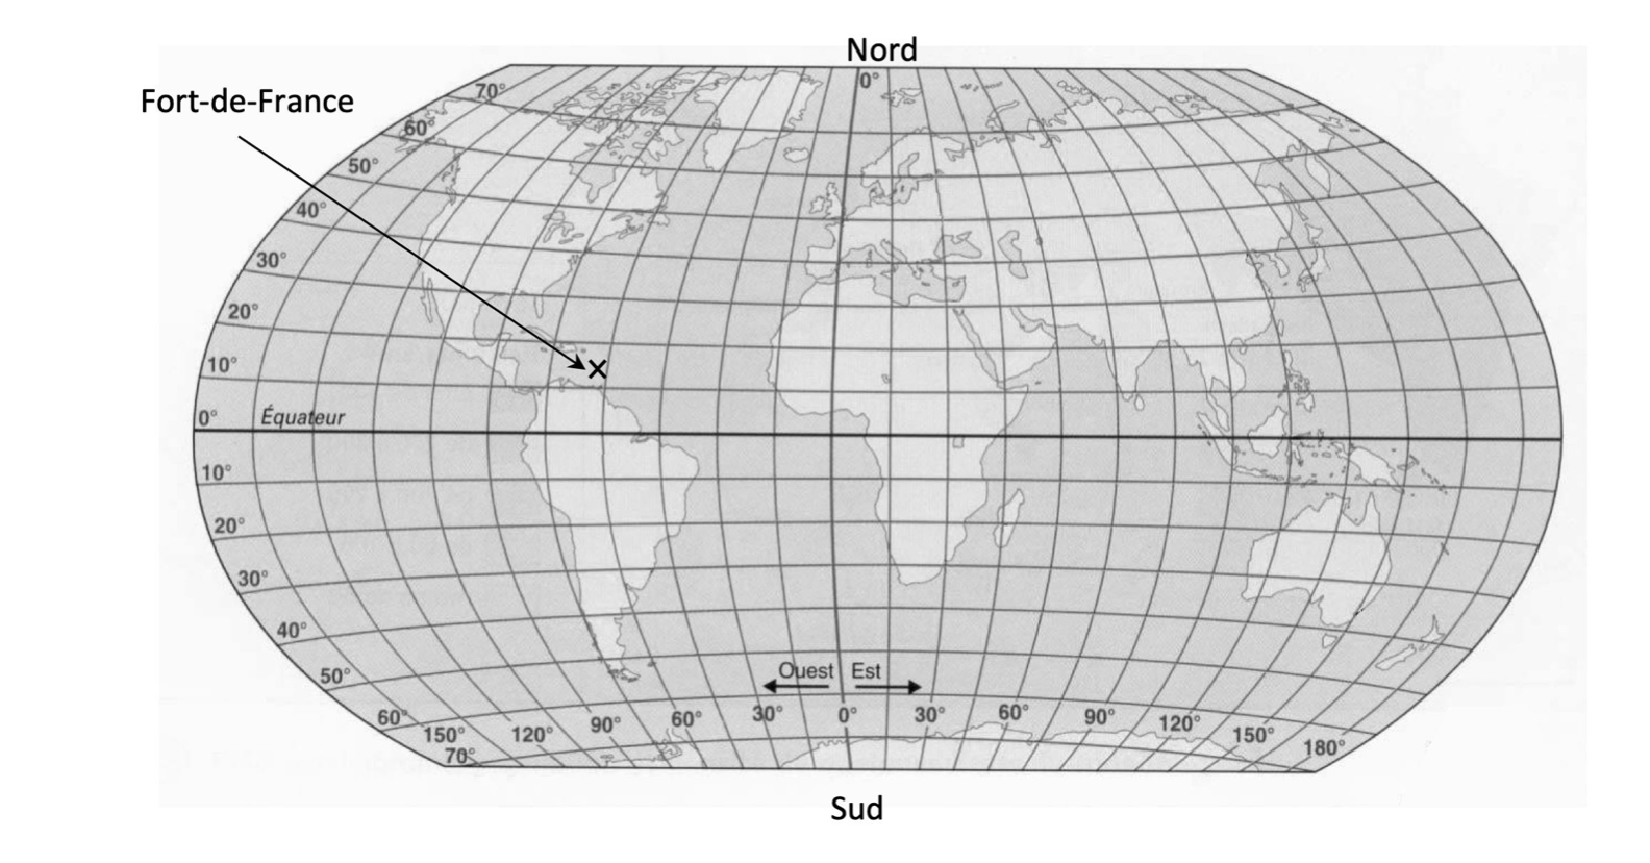
\includegraphics[width=0.9\linewidth]{mappemonde_Poly_sept_2023}
\end{center}

\item Lors de l'édition 2021, $75$ bateaux ont participé à cette course, répartis dans quatre catégories en fonction du parcours à réaliser : Class $40$, Ocean Fifty, Imoca, Ultim.

Le tableau ci-dessous présente les catégories, les effectifs engagés, les distances parcourues et le palmarès de la Transat:

\begin{center}
\begin{tabular}{|l|>{\centering\arraybackslash}m{2cm}|m{2.25cm}|m{2.5cm}|m{3cm}|}\cline{2-5}
\multicolumn{1}{c|}{~}&\textbf{Nombres de bateaux de la catégorie}&\textbf{Distance du parcours}&\textbf{Nom du bateau vainqueur de la catégorie}&\textbf{Durée de course du vainqueur}\\ \hline
\textbf{Class 40}	&43	&\np{4600} milles&Redman	&21 jours 22 heures 33 minutes\\ \hline
\textbf{Ocean Fifty}	&7	&\np{5800} milles&Primonial	&15 jours 13 heures 27 minutes\\ \hline
\textbf{Imoca}		&20	&\np{5800} milles&LinkedOut	&18 jours 1 heure 21 minutes\\ \hline
\textbf{Ultim}		&5	&\np{7500}~milles&Maxi Edmond de Rothschild&16 jours 1 heure 48 minutes\\ \hline
\end{tabular}
\end{center}

\textbf{Information :}

Un mille nautique est une unité de mesure marine qui équivaut à 1,852 km environ.
	\begin{enumerate}
		\item Montrer que le bateau LinkedOut met 2 jours 11 heures et 54 minutes de plus que le bateau Primonial pour effectuer son parcours.
		\item Calculer la moyenne des distances parcourues par l'ensemble des $75$ bateaux. On arrondira cette distance à l'unité près.\index{Moyenne}
		\item La vitesse moyenne du bateau Redman a été d'environ 8,7~milles/h.\index{Vitesse}
		
Montrer que la vitesse moyenne du bateau Maxi Edmond de Rothschild a été environ $2,2$ fois plus grande que celle du bateau Redman.
		\item Un journaliste affirme que la distance parcourue par un bateau de la catégorie Ocean Fifty est environ égale à un quart de périmètre de l'équateur de la Terre.
		
En sachant que le rayon de l'équateur est de \np{6370}~km, le journaliste a-t-il raison ?\index{Longueur du cercle}
	\end{enumerate}
\end{enumerate}

\newpage

\begin{center}
\textbf{\large ANNEXE}

\medskip

\textbf{À compléter et à rendre avec la copie}

\end{center}

\medskip

\textbf{Exercice 2, questions 2. c. et 3. b. :}

\begin{center}
\psset{xunit=1cm,yunit=0.5cm,arrowsize=2pt 3}
\begin{pspicture*}(-5,-13)(6,12)
\psaxes[linewidth=1.25pt,labelFontSize=\scriptstyle]{->}(0,0)(-4.99,-12.99)(6,12)
\psplot[plotpoints=2000,linewidth=1.25pt,linecolor=blue]{-5}{6}{x dup mul x sub 12 sub}
\uput[l](-4.2,10){\blue $\mathcal{C}_f$}
\end{pspicture*}
\end{center}

\bigskip

\textbf{Exercice 3, question 2 :}

\medskip

\begin{scratch}[num blocks]
\initmoreblocks{définir \namemoreblocks{\ovalmoreblocks{Carré}}}
\blockrepeat{répéter \ovalnum{} fois}
{\blockmove{avancer de \ovalmoreblocks{Côté}}
\blockmove{tourner \turnright{} de \ovalnum{} degrés}
}
\end{scratch}
%%%%%%%% fin Polynésie 11 septembre 2023
\newpage
%%%%%%%%   Métropole 18 septembre 2023
\hypertarget{Metropolesep}{}
\label{Metropolesep}

\rfoot{\small Métropole Antilles-Guyane}
\lfoot{\small 18 septembre 2023}
\pagestyle{fancy}
\thispagestyle{empty}
\begin{center}
{\Large\textbf{\decofourleft~ Diplôme national du Brevet
 ~\decofourright}}\\[7pt]
{\Large \textbf{Métropole Antilles-Guyane 18 septembre 2023}}

\vspace{0,5cm}

\textbf{Durée : 2 heures}
\end{center}
\medskip

\framebox[15cm]
{
\begin{minipage}{15cm}
\begin{center}
\textbf{Indications portant sur l'ensemble du sujet.}
\end{center}
Toutes les réponses doivent être justifiées, sauf si une indication contraire est donnée.\\
Pour chaque question, toute trace de  recherche sera prise en compte dans la notation.
\end{minipage}
}
\vspace{0.5cm}

\textbf{{\large \textsc{Exercice 1}} \hfill 20 points}

\medskip

Cet exercice est un questionnaire à choix multiple (QCM).

Pour chaque question, trois réponses (A, B ou C) sont proposées.

\textbf{Une seule réponse est exacte.}

\textbf{Recopier sur la copie le} numéro de la question et la réponse choisie. Aucune justification n’est demandée.

\begin{center}
\begin{tabularx}{\linewidth}{|m{7.5cm}|*{3}{>{\centering \arraybackslash}X|}}\hline
\textbf{Questions}& \textbf{Réponse A}&\textbf{Réponse B}&\textbf{Réponse C}\\ \hline
\textbf{1.~~}Citer trois diviseurs de $84$.&84, 168 et 252& 2, 3 et 4& 2, 5 et 7\\ \hline
\textbf{2.~~}La pyramide SABCD est un agrandissement de coefficient 2 de la pyramide SA$'$B$'$C$'$D$'$.

\begin{minipage}{3.75cm}Par quel nombre doit-on multiplier le volume de la pyramide SA$'$B$'$C$'$D$'$ pour obtenir le volume de la pyramide SABCD ?
\end{minipage}\hfill
\begin{minipage}{3.75cm}
\psset{unit=0.8cm}
\begin{pspicture}(-0.6,-0.5)(4,3.7)
\pspolygon(0,0)(2.7,0)(3.5,0.8)(0,3.2)%ABCSA
\psline(2.7,0)(0,3.2)%BS
\psline(0,1.6)(1.4,1.6)(1.8,2)%A'B'C'
\psline[linestyle=dotted](1.8,2)(0.4,2)(0,1.6)%C'D'A'
\psline[linestyle=dotted](0,0)(0.8,0.8)(3.5,0.8)%ADC
\psline[linestyle=dotted](0.8,0.8)(0,3.2)%DS
\uput[dl](0,0){\footnotesize A} \uput[dr](2.7,0){\footnotesize B} \uput[ur](3.5,0.8){\footnotesize C}
\uput[dr](0.8,0.8){\footnotesize D} \uput[l](0,1.6){\footnotesize A$'$} \uput[dl](1.4,1.6){\footnotesize B$'$}
\uput[ur](1.8,2){\footnotesize C$'$} \uput[ur](0.4,2){\footnotesize D$'$} \uput[u](0,3.2){\footnotesize S}
\end{pspicture}
\end{minipage}&2&8&4\\ \hline
\textbf{3.~~}Quelle est la valeur de l’expression 

$x^2 + 3x - 5$ pour $x  =  - 2$ ?& $- 15$&5&$- 7$\\ \hline
\textbf{4.~~}Dans un sac opaque, on dispose de huit boules numérotées de 1 à 8.

On tire une boule au hasard.

Quelle est la probabilité d’obtenir un multiple de 2 ?&$\dfrac12$&
$\dfrac18$&$\dfrac15$\\ \hline
\textbf{5.~~}Le triangle DEF est l’image du triangle ABC par une homothétie de centre O. Quel est son rapport ?

\psset{unit=0.8cm}
\begin{pspicture}(-2.4,-1)(4.6,1.8)
\pspolygon(-1.1,0)(-0.6,-0.5)(-2.3,-0.5)%ACB
\pspolygon(2.2,0)(4.5,1.1)(1.1,1.1)%DEF
\psdots[dotstyle=+,dotangle=45](0,0)(-1.1,0)(-0.6,-0.5)(-2.3,-0.5)(2.2,0)(4.5,1.1)(1.1,1.1)
\uput[u](-1.1,0){\small A} \uput[d](-2.3,-0.5){\small B} \uput[d](-0.6,-0.5){\small C} \uput[d](2.2,0){\small D} 
\uput[u](4.5,1.1){\small E} \uput[u](1.1,1.1){\small F} \uput[u](0,0){\small O}
\end{pspicture}&$-2$&2&$- \dfrac12$\\ \hline
\end{tabularx}
\end{center}

\newpage

\textbf{{\large \textsc{Exercice 2}} \hfill 14 points}

\medskip

\begin{center}
\psset{unit=0.8cm}
\begin{pspicture}(-1,0)(2.1,1.9)
\pspolygon[linecolor=blue](0,0)(2.1;0)(2.1;60)(2.1;120)
\end{pspicture}
\end{center}

\begin{enumerate}
\item On souhaite tracer le losange ci-dessus de côté $50$ pas à l’aide du bloc losange.

On a écrit le script ci-dessous avec le logiciel Scratch.

Recopier les lignes 3 et 6 sur la copie en les complétant.

\begin{center}
\begin{scratch}[num blocks]
\initmoreblocks{définir \namemoreblocks{losange}}
\blockpen{stylo en position d'écriture}
\blockrepeat{répéter \ovalnum{...} fois}
{
\blockmove{avancer de \ovalnum{50} pas}
\blockmove{tourner \turnright{} de \ovalnum{60} degrés}
\blockmove{avancer de \ovalnum{...} pas}
\blockmove{tourner \turnright{} de \ovalnum{120} degrés}
}
\blockpen{relever le stylo}
\end{scratch}
\end{center}

\item Préciser sur votre copie quelle figure est associée à chaque script 1, 2 ou 3.

Aucune justification n’est demandée.

\begin{center}
\begin{tabularx}{\linewidth}{*{3}{>{\centering \arraybackslash}X}}
Figure A &Figure B& Figure C\\ \hline
\psset{unit=0.3cm}
\begin{pspicture}(-3,0)(6.1,1.9)
\def\los{\pspolygon[linecolor=blue](0,0)(2.1,0)(1.2,1.8)(-0.9,1.8)}
\multido{\n=-3.0+3}{4}{\rput(\n,0){\los}}
\end{pspicture}&
\psset{unit=0.25cm}
\begin{pspicture}(-3,-1)(7.6,5)
\def\los{\pspolygon[linecolor=blue](0,0)(2.1,0)(1.2,1.8)(-0.9,1.8)}
\multido{\n=-3+2.1,\na=-0.5+1.0}{4}{\rput(\n,\na){\los}}
\end{pspicture}&
\psset{unit=0.3cm}
\begin{pspicture}(-3,0)(5,3.9)
\def\los{\pspolygon[linecolor=blue](0,0)(2.1,0)(1.2,1.8)(-0.9,1.8)}
\multido{\n=-2.0+2.1}{4}{\rput(\n,0){\los}}
\end{pspicture}\\
Script 1 &Script 2 &Script 3\\
\setscratch{scale=.8}
\begin{scratch}
\blockinit{Quand \ovalnum{1} est pressé}
\blockmove{aller à x: \ovalnum{-220} y: \ovalnum0}
\blockmove{s'orienter à \ovalnum{\selectmenu{90}} degrés}
\blockpen{effacer tout}
\blockrepeat{répéter \ovalnum{4} fois}
{\blockmove{losange}
\blockmove{avancer de \ovalnum{50} pas}
}
\end{scratch}&
\setscratch{scale=.8}
\begin{scratch}
\blockinit{Quand \ovalnum{2} est pressé}
\blockmove{aller à x: \ovalnum{-220} y: \ovalnum0}
\blockmove{s'orienter à \ovalnum{\selectmenu{90}} degrés}
\blockpen{effacer tout}
\blockrepeat{répéter \ovalnum{4} fois}
{\blockmove{losange}
\blockmove{avancer de \ovalnum{100} pas}
}
\end{scratch}&
\setscratch{scale=.8}
\begin{scratch}
\blockinit{Quand \ovalnum{3} est pressé}
\blockmove{aller à x: \ovalnum{-220} y: \ovalnum0}
\blockmove{s'orienter à \ovalnum{\selectmenu{90}} degrés}
\blockpen{effacer tout}
\blockrepeat{répéter \ovalnum{4} fois}
{\blockmove{losange}
\blockmove{avancer de \ovalnum{50} pas}
\blockmove{ajouter \ovalnum{30} à y}
}
\end{scratch}\\
\end{tabularx}
\end{center}
\item  Dans la figure ci-dessous obtenue par le programme associé, décrire une transformation qui permet d’obtenir le losange ABCD à partir du losange EDCF.

Préciser ses caractéristiques.

%\begin{tabularx}{\linewidth}{*{2}{>{\centering \arraybackslash}X}}
\begin{minipage}{7cm}
\psset{unit=1cm}
\begin{pspicture}(-2.8,-2.8)(2.8,2.8)
\def\los{\pspolygon[linecolor=blue](0,0)(1.4;0)(2.42488;30)(1.4;60)}
\multido{\n=0+60}{6}{\rput{\n}(0,0){\los}}
\uput[u](2.42488;90){A} \uput[ur](1.4;60){B} \uput[d](0,-0.1){C}
\uput[ul](1.4;120){D} \uput[ul](2.42488;150){E} \uput[l](1.4;180){F} 
\end{pspicture}
\end{minipage}\hfill
\begin{minipage}{7cm}
\begin{scratch}
\blockinit{Quand \greenflag est cloqué}
\blockpen{effacer tout}
\blockmove{aller à x: \ovalnum{0} y: \ovalnum0}
\blockrepeat{répéter \ovalnum{6} fois}
{\blockmove{losange}
\blockmove{tourner \turnright{} de \ovalnum{60} degrés}}
\end{scratch}
\end{minipage}
%\end{tabularx}
\end{enumerate}

\newpage

\textbf{{\large \textsc{Exercice 3}} \hfill 22 points}

\medskip

Une piscine propose deux tarifs d'entrée pour l'année 2023.

\textbf{Tarif A} : $5,90$~\euro{} l'entrée.

\textbf{Tarif B} : $4,40$~\euro{} l'entrée avec une carte d'abonnement de $30$~\euro{} valable toute l'année.

\medskip

\begin{enumerate}
\item 
	\begin{enumerate}
		\item Quel est le prix total pour $10$ entrées avec le tarif A ?
		\item Quel est le prix total pour $10$ entrées avec le tarif B ?
	\end{enumerate}
\item  On note $f$ et $g$ les fonctions qui modélisent les prix, en euro, respectivement du tarif A et du tarif B en fonction du nombre $x$ d'entrées.

Donner l'expression de $f(x)$, puis celle de $g(x)$.
\item 
	\begin{enumerate}
		\item Résoudre l'équation $5,90x = 4,40x + 30$.
		\item Quel est le nombre d'entrées pour lequel les tarifs A et B donnent le même prix à payer ?
	\end{enumerate}
\end{enumerate}

On relève le nombre d'entrées par mois durant une année.

\begin{center}
\begin{tabularx}{\linewidth}{|m{1.5cm}|*{12}{>{\centering \arraybackslash \footnotesize}X|}}\hline
\footnotesize Mois	&Jan.	& Fév.& Mars& Avril& Mai& Juin& Juillet& Août& Sept.& Oct.& Nov.& Déc.\\ \hline
\footnotesize 
Nombre d'entrées	&\np{12500} &\np{13700} &\np{10400} &\np{13600} &\np{12300} &\np{11700} &\np{10400} &\np{11600} &\np{10200} &\np{13800} &\np{12600} &\np{11800}\\ \hline
\end{tabularx}
\end{center}
\begin{enumerate}[resume]
\item
	\begin{enumerate}
		\item Calculer le nombre moyen d'entrées par mois.
		\item Calculer l'étendue du nombre d'entrées par mois.
	\end{enumerate}
\item La piscine a la forme d'un pavé droit de longueur $50$~m, de largeur $25$~m et de profondeur $3$~m. En admettant qu'elle soit entièrement remplie, déterminer en m$^3$, le volume d'eau qui sera évacué pour réaliser la vidange.
\end{enumerate}

\bigskip

\textbf{{\large \textsc{Exercice 4}} \hfill 20 points}

\medskip

Un funiculaire est un type de transport en commun circulant sur des rails et dont la traction est assurée par câble. Il est généralement utilisé pour des lignes comportant des fortes pentes.

Les documents suivants permettent de répondre aux questions.

\medskip

\textbf{Document 1 : tarifs du funiculaire}

\begin{center}
\begin{tabularx}{\linewidth}{|m{4.2cm}|m{2cm}|m{4.2cm}|X|}\hline
\multicolumn{2}{|c|}{Tarif individuel}& \multicolumn{2}{|c|}{Tarif de groupe à partir de 20 personnes}\\
\multicolumn{2}{|c|}{(tarif enfant accordé pour les enfants }& \multicolumn{2}{|c|}{(adultes et enfants)}\\
\multicolumn{2}{|c|}{de 5 à 11 ans)}& \multicolumn{2}{|c|}{}\\ \hline
Aller simple par adulte&8 euros		&Aller simple par adulte&7 euros\\ \hline
Aller-retour par adulte&10 euros	&Aller-retour par adulte&8,50 euros\\ \hline
Aller simple par enfant&6,50 euros	&Aller simple par enfant &5,50 euros\\ \hline
Aller-retour par enfant&8 euros		&Aller-retour par enfant&7 euros\\ \hline
\end{tabularx}
\end{center}

\textbf{Document 2 : trajet du funiculaire vu de profil}

\begin{center}
\psset{unit=1cm,arrowsize=2pt 3}
\begin{pspicture}(15,5.5)
\psline(0.5,0)(10.7,0)(10.7,4)%DEB
\psline[linewidth=1.25pt](10.7,4)(6.8,2.9)(0.5,0)%BAD
\psline[linestyle=dashed](6.8,2.9)(10.7,2.9)%AC
\psline[linewidth=0.6pt]{<->}(0.3,0.6)(6.6,3.5)\rput{24.7}(3.45,2.25){448,5 m}
\psline[linewidth=0.6pt]{<->}(11.5,2.9)(11.5,4)\uput[r](11.5,3.45){Dénivelée : 50 m}
\uput[d](8.75,2.9){\small Longueur horizontale}
\psframe(10.7,2.9)(10.4,3.2)
\uput[ul](6.8,2.9){A} \uput[u](10.7,4){B} \uput[dr](10.7,2.9){C} \uput[dl](0.5,0){D} \uput[dr](10.7,0){E} 
\end{pspicture}
\end{center}

\begin{enumerate}
\item Un groupe constitué de 12 adultes et de 8 enfants (âgés de 6 à 10 ans) fait un aller-retour en funiculaire.
	\begin{enumerate}
		\item Quel est le prix à payer par le groupe en utilisant le tarif individuel ?
		\item Quel est le prix à payer par le groupe en utilisant le tarif de groupe ?
		\item Déterminer le pourcentage de la réduction obtenue en appliquant le tarif groupe par rapport au tarif individuel.
	\end{enumerate}
\item Sur la première partie du trajet [DA], le funiculaire parcourt $448,5$~m en 8~min 45~s.

Quelle est sa vitesse moyenne en mètres par seconde ?

On donnera le résultat au centième près.
\item Sur la dernière partie du trajet [AB], la pente est de 25\,\% et la dénivelée BC est de $50$~m, calculer la longueur horizontale AC.
\end{enumerate}

\emph{Définition} : Pente $= \dfrac{\text{Dénivelée}}{\text{Longueur horizontale}}$

\bigskip

\textbf{{\large \textsc{Exercice 5}} \hfill 24 points}

\medskip

\emph{La figure ci-dessous n'est pas à l'échelle}

\begin{center}
\psset{unit=1cm,arrowsize=2pt 3}
\begin{pspicture}(-1.5,-1)(12,7.4)
%\psgrid
\pspolygon[linewidth=1.25pt](0,0)(9.3,0)(2.2,5)%BCA
\psline[linewidth=1.25pt](2.2,5)(2.2,0)%AH
\psline[linewidth=1.25pt](1.03,2.4)(5.9,2.4)%MN
\psframe(2.2,0)(2.5,0.3)
\psline[linewidth=0.6pt]{<->}(-1,0.45)(0,2.85)\rput{67.4}(-0.65,1.85){2,5 cm}
\psline[linewidth=0.6pt]{<->}(0,2.85)(1.2,5.45)\rput{67.4}(0.35,4.35){2,7 cm}
\psline[linewidth=0.6pt]{<->}(3,6)(10.1,1)\rput{-35.15}(6.55,3.75){8,5 cm}
\psline[linewidth=0.6pt]{<->}(0,-0.8)(2.2,-0.8)\uput[d](1.1,-0.8){2 cm}
\uput[u](2.2,5){A} \uput[l](1.03,2.4){M} \uput[ur](5.9,2.4){N}
\uput[dl](0,0){B} \uput[d](2.2,0){H} \uput[dr](9.3,0){C}
\end{pspicture}
\end{center}

Dans le triangle ABC ci-dessus, M est un point du côté [AB], N est un point du côté [AC], et H est un point du côté [BC] ; les droites (MN) et (BC) sont parallèles.

On donne :
\begin{itemize}
\item[$\bullet$~~] AC $ = 8,5$~cm ;
\item[$\bullet$~~] AM $ = 2,7$~cm ;
\item[$\bullet$~~] MB $ = 2,5$~cm ;
\item[$\bullet$~~] BH $ = 2$~cm.
\end{itemize}

On rappelle que toutes les réponses doivent être justifiées.

\medskip

\begin{enumerate}
\item Calculer AB.
\item Montrer que la longueur AH est égale à $4,8$~cm.
\item Calculer la mesure de l'angle $\widehat{\text{ACH}}$. Arrondir au degré près.
\item Calculer la longueur HC. Arrondir au cm près.
\item Un élève affirme que: \og AN est inférieure à $4$~cm \fg. A-t-il raison ?
\item Calculer l'aire du triangle AHC.
\end{enumerate}
%%%%%%%%%  fin Métropole 18 septembre 2023
\newpage
%%%%%  Amérique du Sud 16 novembre 2023 
\hypertarget{AmeriqueSud}{}

\label{AmeriqueSud}

\lfoot{\small{Amérique du Sud}}
\rfoot{\small{16 novembre 2023}}
\pagestyle{fancy}
\thispagestyle{empty}
\begin{center}

{\Large \textbf{\decofourleft~Brevet des collèges Amérique du Sud 16 novembre 2023~\decofourright}}

\bigskip

\textbf{Durée : 2 heures}

\end{center}

\bigskip

\textbf{\large Exercice 1 \hfill 20 points}

\bigskip

\begin{minipage}{7.5cm}
On considère la figure ci-contre dans laquelle:

\begin{itemize}
\item[$\bullet$~] Les points F{}, G et H sont alignés
\item[$\bullet$~] (LH) est perpendiculaire à (FH)
\item[$\bullet$~] EF $= 18$ cm ; FG $= 24$ cm ; EG $= 30$ cm ;

GH = $38,4$ cm
\item[$\bullet$~] $\widehat{\text{EGF}} = \widehat{\text{LGH}}$.
\end{itemize}
\end{minipage}\hfill
\begin{minipage}{7.5cm}
\psset{unit=1cm}
\begin{pspicture}(7.8,4.8)
\pspolygon(0.2,3.8)(0.2,1)(7.5,1)(7.5,4.6)(3.3,1)
\pswedge*(3.3,1){0.4}{0}{39}
\pswedge*(3.3,1){0.4}{141}{180}
\psframe(7.5,1)(7.2,1.3)
\rput(3.9,0.2){\emph{La figure n'est pas en vraie grandeur.}}
\uput[u](0.2,3.8){E} \uput[dl](0.2,1){F} \uput[d](3.3,1){G} \uput[dr](7.5,1){H}\uput[ur](7.5,4.6){L}
\end{pspicture}
\end{minipage}

\begin{enumerate}
\item Montrer que le triangle EFG est rectangle en F{}.\index{Réciproque de Pythagore}
\item Calculer la mesure de l'angle $\widehat{\text{EGF}}$.\index{Trigonométrie}

Donner l'arrondi au degré près.
\item Montrer que les triangles EGF et LGH sont semblables.\index{Triangles semblables}
\item Parmi les propositions suivantes, quel est le coefficient d'agrandissement qui permet de
passer du triangle EFG au triangle LHG ?\index{Agrandissement}

Expliquer.

\begin{center}
\begin{tabularx}{0.75\linewidth}{|*{4}{>{\centering \arraybackslash}X|}}\hline
0,625 &1,28	& 1,6	&2,6\\ \hline
\end{tabularx}
\end{center}

\item Quel est le périmètre du triangle LGH ?
\end{enumerate}

\medskip

\textbf{\large Exercice 2 \hfill 21 points}

\medskip

\begin{minipage}{8cm}
À partir d'une feuille rectangulaire de dimension $10$~cm sur $8$~cm, on coupe les quatre coins de manière identique.

On obtient ainsi un polygone FELKJIHG et quatre triangles rectangles isocèles égaux comme représenté ci-contre.

AD $= 10$ cm ; AB $= 8$ cm.
\end{minipage} \hspace{0.5cm}
\begin{minipage}{7.2cm}
\psset{unit=1cm}
\begin{pspicture}(7.2,6.5)
\def\barbar{\psline(-0.05,-0.1)(-0.05,0.1)\psline(0.05,-0.1)(0.05,0.1)}
\psline[linestyle=dashed](2.1,5.6)(0.3,3.8)
\psline[linestyle=dashed](0.3,2.4)(2.1,0.6)
\psline[linestyle=dashed](4.7,0.6)(6.5,2.4)
\psline[linestyle=dashed](6.5,3.8)(4.7,5.6)
\psframe[linewidth=1.5pt](0.3,0.6)(6.5,5.6)
\rput(1.2,5.6){\barbar}\rput(5.6,5.6){\barbar}
\rput(1.2,0.6){\barbar}\rput(5.6,0.6){\barbar}
\rput{90}(0.3,4.7){\barbar}\rput{90}(0.3,1.5){\barbar}
\rput{90}(6.5,4.7){\barbar}\rput{90}(6.5,1.5){\barbar}
\rput{-45}(1.2,1.5){\Large \ding{36}}
\uput[ul](0.3,5.6){A} \uput[dl](0.3,0.6){B} \uput[dr](6.5,0.6){C} \uput[ur](6.5,5.6){D}
\uput[u](2.1,5.6){E} \uput[l](0.3,3.8){F} \uput[l](0.3,2.4){G} \uput[d](2.1,0.6){H}
\uput[d](4.7,0.6){I} \uput[r](6.5,2.4){J} \uput[r](6.5,3.8){K} \uput[u](4.7,5.6){L}
\end{pspicture}
\end{minipage}

\medskip

\textbf{Les deux parties sont indépendantes.}

\medskip

\textbf{Première partie : on suppose que AE = 3 cm.}

\begin{enumerate}
\item Quelle est l'aire du triangle AEF ?\index{Aire du triangle}
\item En déduire l'aire du polygone FELKJIHG.
\end{enumerate}

\medskip

\textbf{Deuxième partie :}

On souhaite que l'aire du polygone FELKJIHG soit de 60 cm$^2$.

Pour cela, on fait varier la longueur AE et on observe l'effet sur l'aire du polygone FELKJIHG.

On note $x$ la longueur AE exprimée en cm.

\begin{enumerate}[resume]
\item 
	\begin{enumerate}
		\item Exprimer l'aire du triangle AEF en fonction de $x$.\index{Aire du triangle}
		\item Montrer que l'aire du polygone FELKJIHG, en cm$^2$, est donnée par l'expression $80 - 2x^2$.
	\end{enumerate}
\item On considère la fonction $f : x \longmapsto ~80 - 2x^2$.

À l'aide d'un tableur, on a produit le tableau de valeurs ci-dessous :\index{Tableur}
\begin{center}
\begin{tabularx}{0.9\linewidth}{|c|*{10}{>{\centering \arraybackslash}X|}}\hline
&A&B&C&D & E&F& G& H&I&J\\ \hline
1&$x$&0&0,5&1&1,5&2& 2,5&3&3,5& 4\\ \hline
2&$f(x)$&80&79,5&78&45,5&72& 67,5& 62&55,5& 48\\ \hline
\end{tabularx}
\end{center}

Proposer une formule qui a pu être saisie en B2 avant d'être étirée vers la droite.

Ne pas justifier.
\item Voici la courbe représentative de la fonction $f$ :
\begin{center}
\psset{xunit=2.2cm,yunit=0.1cm,comma=true}
\begin{pspicture}(4.5,90)
\multido{\n=0.0+0.5}{10}{\psline[linewidth=0.2pt](\n,0)(\n,90)}
\multido{\n=0+10}{10}{\psline[linewidth=0.2pt](0,\n)(4.5,\n)}
\psaxes[linewidth=1.25pt,Dx=0.5,Dy=10]{->}(0,0)(4.5,90)
\uput[d](4.4,0){$x$}\uput[l](0,87){$f(x)$}
\psplot[plotpoints=2000,linewidth=1.25pt,linecolor=blue]{0}{4.5}{80 x dup mul 2 mul sub}
\end{pspicture}
\end{center}
\medskip

	\begin{enumerate}
		\item La fonction $f$ est-elle affine ?\index{Fonction affine}
		\item Par lecture graphique, déterminer une valeur approchée de la longueur AE permettant d'obtenir un polygone FELKJIHG d'aire égale à 60 cm$^2$.\index{Lecture graphique}
		\item Trouver par le calcul la valeur exacte de cette longueur.
	\end{enumerate}
\end{enumerate}

\bigskip

\textbf{\large Exercice 3 \hfill 20 points}

\medskip

\textbf{Pour chacune des affirmations, indiquer si elle est vraie ou fausse en justifiant la réponse.}\index{Vrai-Faux}

\medskip

\begin{enumerate}
\item On considère le tableau ci-dessous :
\begin{center}
\begin{tabularx}{0.8\linewidth}{|l|*{4}{>{\centering \arraybackslash}X|}}\hline
Nombre de baguettes &1 &2 &3 &4 \\ \hline
Prix en \euro{}& 1,10& 2,20& 3,30& 4\\ \hline
\end{tabularx}
\end{center}

\textbf{Affirmation 1 :} \og Le prix est proportionnel au nombre de baguettes. \fg\index{Proportionnalité}

\item On considère ci-dessous le point A sur une droite graduée:

\begin{center}
\psset{xunit=5cm,arrowsize=2pt 3}
\begin{pspicture}(0.75,-0.25)(2.75,0.25)
\psaxes[linewidth=2pt,ticks=x,subticks=8,xsubticksize=2,Ox=1](1,0)(0.75,0.)(2.5,0.0)
\uput[u](2.25,0){A}
\end{pspicture}
\end{center}

\textbf{Affirmation 2 :} \og L'abscisse du point A est un nombre décimal. \fg

\item \begin{minipage}{7.5cm}
On considère cet engrenage qui est composé d'une roue A à 8 dents et d'une roue B à 12 dents.

\textbf{Affirmation 3 :}

\og Cet engrenage sera dans la même position au bout de 6 tours pour la roue A et de 4 tours pour la roue B. \fg
\end{minipage}
\begin{minipage}{7.5cm}
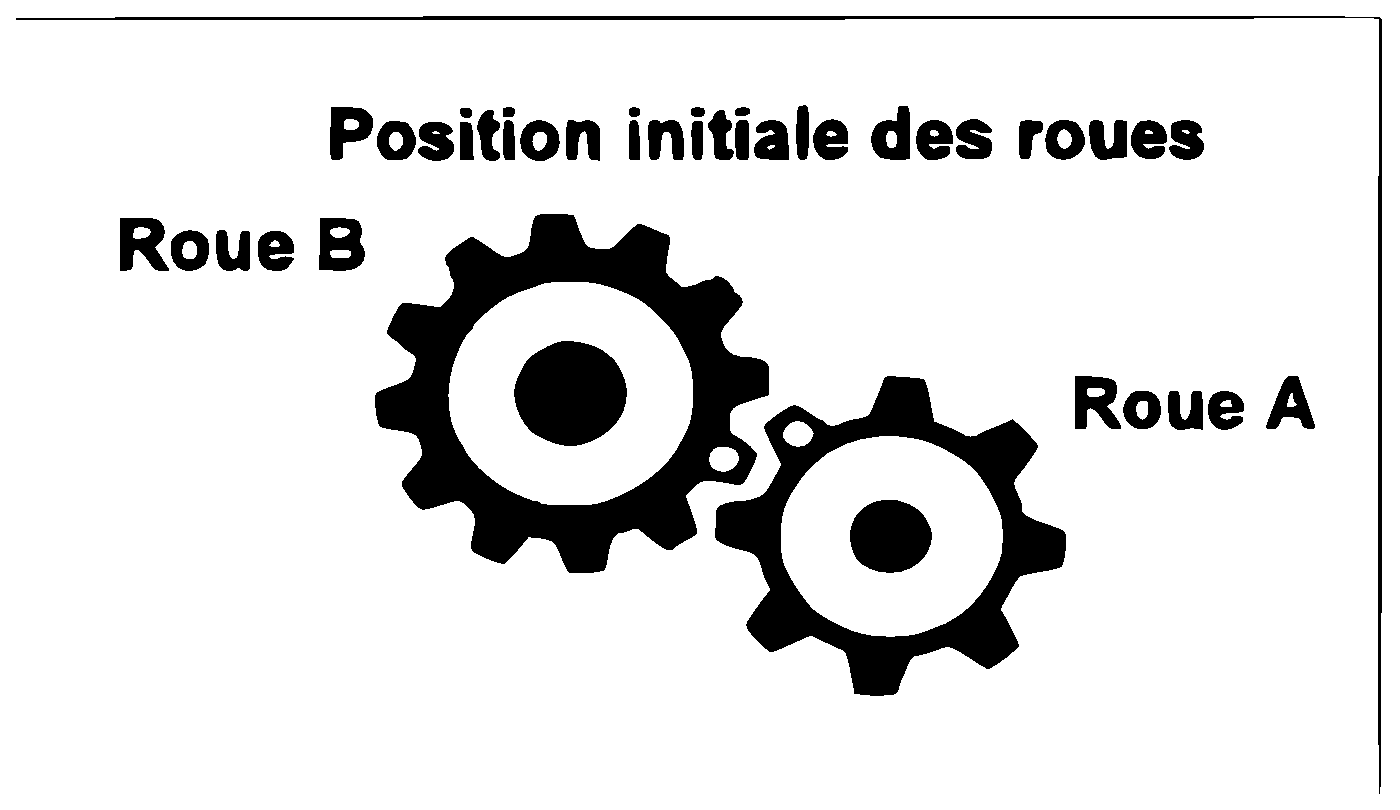
\includegraphics[width=6cm]{engrenages}
\end{minipage}

\item \textbf{Affirmation 4 :}

\og Pour tout nombre $x$, l'égalité suivante est vraie:
\begin{center}$(x + 8)(2x - 1) = 2x^2 -(8 - 15x)$.\fg\end{center}
\end{enumerate}

\medskip

\textbf{\large Exercice 4 \hfill 16 points}

\medskip

Une usine fabrique des bougies parfumées en cire de forme cylindrique.

\medskip

\textbf{Les questions 1, 2 et 3 sont indépendantes}

\begin{center}
\begin{tabularx}{\linewidth}{|p{5.8cm}|X|}\hline
\textbf{Document 1}

\psset{unit=1cm,arrowsize=2pt 3}
\begin{pspicture}(-2.7,0)(2.7,4.9)
\psellipse(0,4)(0.7,0.15)
\psellipticarc(0,0.8)(0.7,0.15){180}{0}
\psellipticarc[linestyle=dashed](0,0.8)(0.7,0.15){0}{180}
\psline(-0.7,0.8)(-0.7,4)\psline(0.7,0.8)(0.7,4)
\pscurve[linewidth=1.5pt](0,4)(-0.1,4.15)(0.15,4.3)
\rput(1.,4.4){la mèche}\rput(1.9,2.35){la bougie}
\psline{<->}(0,0.5)(0.7,0.5)
\uput[d](0.35,0.5){\small 3 cm}
\psline{<->}(-1,0.8)(-1,4)
\uput[l](-1,2.4){\small 12 cm}
\end{pspicture}

Rayon du cylindre : 3 cm 

Hauteur du cylindre : 12 cm&
\textbf{Document 2}

Aire d'un disque  : rayon $^2 \times \pi$

Volume d'un cylindre : Aire de la base $\times$ hauteur
%\rule{6cm}

\textbf{Document 3}

\begin{itemize}
\item Une bougie est composée de cire et de parfum.
\item Le volume de cire nécessaire à la fabrication d'une bougie correspond au $\dfrac{9}{10}$ du volume de cette bougie.
\item 1~cm$^3$ de cire a une masse de $0,7$~g.
\end{itemize}\\ \hline
\end{tabularx}
\end{center}

\begin{enumerate}
\item 
	\begin{enumerate}
		\item Montrer que le volume d'une bougie est d'environ 339 cm$^2$.\index{Volume du cylindre}
		\item Quelle est la masse de cire nécessaire pour une bougie ? On donnera une valeur approchée au gramme près.
	\end{enumerate}

\begin{minipage}{8.4cm}
\item Au mois de novembre, l'usine a fabriqué des bougies de 4 parfums différents:

vanille, miel, lavande et jasmin.

Le diagramme circulaire codé ci-contre donne la répartition, pour le mois de novembre, du nombre de bougies fabriquées en fonction de leur parfum.\index{Diagramme circulaire}

Les bougies au miel représentent 22\,\% de la production du mois de novembre.

Quel est le pourcentage de bougies à la lavande fabriquées au mois de novembre ?\index{Pourcentage}
\end{minipage}\hspace{0.4cm}
\begin{minipage}{4.8cm}
\psset{unit=0.8cm}
\begin{pspicture}(-2.9,-2.9)(2.9,2.9)
\pscircle(0,0){2.9}
\psline(2.9;180)(0,0)(2.9;-90)
\psline(2.9;5.4) \psline(2.9;84.6)
\rput(1.45;46){Miel}\rput(1.45;135){Lavande}
\rput(1.45;225){Vanille}\rput(1.45;-45){Jasmin}
\psframe(0,0)(-0.3,-0.3)
\psarc(0,0){0.5}{5.4}{84.6}\psarc(0,0){0.6}{5.4}{84.6}
\psarc(0,0){0.4}{84.6}{180}\psarc(0,0){0.4}{270}{5.4}
\end{pspicture}
\end{minipage}

\item Durant les trois premiers mois de l'année suivante, l'entreprise se donne pour objectif de produire en moyenne \np{7900} bougies par mois.

En janvier, elle fabrique \np{6500} bougies et \np{8000} en février.

Quel est le nombre de bougies à produire en mars pour atteindre l'objectif ?\index{Moyenne}
\end{enumerate}

\medskip

\textbf{\large Exercice 5 \hfill 23 points}

\medskip

On dispose d'une roue dont les 4 secteurs ont tous la même aire et sont numérotés : 

1 ; 2 ; 3 ;~4.

On dispose également d'une urne contenant 3 boules numérotées: 2 ; 3 et 4.

Les boules sont indiscernables au toucher.

On considère l'expérience aléatoire suivante : 

\og On fait tourner la roue puis on tire au hasard une boule dans l'urne. On forme alors un nombre entier à deux chiffres tel que :

\begin{itemize}
\item[$\bullet~~$]Le chiffre des dizaines est le numéro indiqué par la flèche sur la roue.
\item[$\bullet~~$]Le chiffre des unités est le numéro de la boule tirée dans l'urne. \fg
\end{itemize}

\psset{unit=1cm,arrowsize=2pt 3}
\begin{center}
\begin{pspicture}(13.5,4)
%\psgrid
\pscircle(4.5,2.2){1.3}
\rput(3.9,3){1} \rput(3.9,3){1} \rput(5.2,3){4} \rput(5.2,1.5){3} \rput(3.9,1.5){2}
\rput(4.5,0.4){La roue: chiffre des dizaines}
\psline[linewidth=2.5pt]{->}(3,4)(3.7,3.22)
\pspolygon(10,0.8)(12.6,0.8)(12.1,3.3)(10.5,3.3)
\rput(11.4,0.4){L'urne: chiffre des unités}
\pscircle(10.8,1.6){0.4} \pscircle(11.8,1.6){0.4}\pscircle(11.4,2.6){0.4}
\rput(10.8,1.6){2} \rput(11.8,1.6){4} \rput(11.4,2.6){3}
\end{pspicture}
\end{center}

\emph{Exemple} : Si la flèche indique le numéro 1 sur la roue et que la boule tirée dans l'urne porte le numéro 3, on forme le nombre 13.

\medskip

\begin{enumerate}
\item Écrire la liste des 12 issues possibles.
\item Déterminer la probabilité de l'évènement: \og Obtenir un nombre impair \fg.
\item On considère l'évènement $A$ : \og Le nombre formé est un nombre premier et inférieur à 30 \fg.
	\begin{enumerate}
		\item Quelle est la probabilité de l'évènement $A$ ?\index{Probabilité}
		\item Quelle est la probabilité de son évènement contraire ?\index{Evènement contraire@Évènement contraire}
	\end{enumerate}
\end{enumerate}

À l'aide de cette expérience aléatoire, on crée un jeu de hasard.

Le joueur gagne s'il obtient un multiple de 11.\index{Multiple}

\begin{enumerate}[resume]
\item Montrer que la probabilité d'obtenir un multiple de 11 est égale à $0,25$.
\item On souhaite simuler ce jeu à l'aide d'un logiciel de programmation.

On a rédigé le script ci-dessous:\index{Scratch}

\begin{center}
\setscratch{scale=.8}
\begin{scratch}[num blocks]
\blockinit{quand \greenflag est cliqué}
\blockvariable{mettre \ovalcontrol*{Gagné} à \ovalnum{0}}
\blockrepeat{répéter \ovalnum{100} fois}
{%% début repeat
\blockvariable{mettre \ovalcontrol*{Chiffre des dizaines} à \ovaloperator{nombre aléatoire entre \ovalnum{1} et \ovalnum{4}}}
\blockvariable{mettre \ovalcontrol*{Chiffre des unités} à \ovaloperator{nombre aléatoire entre \ovalnum{...} et \ovalnum{...}}}
\blockif{si \ovalnum{....................} = \ovalnum{....................} alors}
{%% début if
\blockvariable{ajouter \ovalnum{1} à \ovalnum{Gagné}}
}%% fin if
}%% fin repeat
\blockstop{dire  regrouper \ovalnum{La fréquence d'apparition d'un multiple de 11 est de :} et \ovalcontrol{Gagné} / \ovalnum{100} pendant \ovalnum{2} secondes}
\end{scratch}
\end{center}

Information:

\ovaloperator{nombre aléatoire entre \ovalnum{1} et \ovalnum{4}} renvoie au hasard un nombre parmi 1, 2, 3, 4.
	\begin{enumerate}
		\item Écrire sur la copie comment compléter les deux cases vides de la ligne 5.

\emph{Ne pas justifier}.
		\item Écrire sur la copie comment compléter les deux cases vides de la ligne 6.

\emph{Ne pas justifier}.
		\item On a cliqué sur le drapeau et voici le résultat du programme :

\og La fréquence d'apparition d'un multiple de $11$ est $0,23$. \fg

Pourquoi le résultat est-il différent de celui obtenu dans la question 4 ?
	\end{enumerate}
\end{enumerate}
%%%%%%%   fin Amérique du Sud 16 novembre 2023
\newpage
%%%%%%%   Nouvelle-Calédonie 7 décembre 2023
\hypertarget{Caledoniedec}{}

\label{Caledoniedec}

\lfoot{\small{Nouvelle-Calédonie}}
\rfoot{\small{7 décembre 2023}}
\marginpar{\rotatebox{90}{\textbf{A. P{}. M. E. P{}.}}}
\pagestyle{fancy}
\thispagestyle{empty}

\begin{center}\textbf{Durée : 2 heures}

\vspace{0,5cm}

{\Large\textbf{\decofourleft~Diplôme national du Brevet
Nouvelle--Calédonie~\decofourright}}\\[7pt]
{\Large \textbf{7 décembre 2023}}
\end{center}

\vspace{0,5cm}

\textbf{Exercice 1 : Q. C. M.\hfill 15 points}

\medskip

Cet exercice est un questionnaire à choix multiples (QCM).\index{QCM}

Pour chaque question, une seule des trois réponses proposées est exacte.

\textbf{Sur la copie, indiquer le numéro de la question et la réponse A, B ou C choisie.\\
Aucune justification n'est demandée.}

Aucun point ne sera enlevé en cas de mauvaise réponse.

\begin{center}
\begin{tabularx}{\linewidth}{|c|m{8cm}|*{3}{>{\centering \arraybackslash}X|}}\hline
&\textbf{Questions}&\textbf{Réponse A}&\textbf{Réponse B}&\textbf{Réponse C}\\ \hline
1 &D'après des chercheurs, la probabilité qu'une personne subisse une attaque mortelle par un requin au cours de sa vie, est de ...&$2,7 \times 10^{-7}$&$2,7\times 10^0$&$2,7 \times 10^7$\\ \hline
2&$\dfrac35 - \dfrac25 \times \dfrac74$\rule[-4mm]{0mm}{10mm}&$- \dfrac{1}{10}$&$\dfrac{2}{10}$&$\dfrac{7}{20}$\rule[-4mm]{0mm}{10mm}\\ \hline
3&Sur un site, un pantalon est vendu 60~\euro{} au lieu de 80~\euro.

Le pourcentage de réduction est ...&20\,\%&25\,\%&75\,\%\\ \hline\index{Pourcentage}
4&ABCD est un parallélogramme de centre E.

\begin{center}
\psset{unit=1cm}
\begin{pspicture}(7.4,2.3)
\pspolygon(0.4,0.3)(5.5,0.3)(7.1,2.1)(2,2.1)%ADCB
\psline(0.4,0.3)(7.1,2.1)\psline(5.5,0.3)(2,2.1)
\psdots(1.2,1.2)(2.95,0.3)
\uput[dl](0.4,0.3){A} \uput[ul](2,2.1){B} \uput[ur](7.1,2.1){C} \uput[dr](5.5,0.3){D} \uput[u](3.75,1.2){E} \uput[d](1.2,1.2){F}\uput[d](2.95,0.3){G}
\psline(1.65,0.2)(1.65,0.4)\psline(1.7,0.2)(1.7,0.4)\psline(1.75,0.2)(1.75,0.4)
\psline(4.2,0.2)(4.2,0.4)\psline(4.25,0.2)(4.25,0.4)\psline(4.3,0.2)(4.3,0.4)
\rput(0.8,0.75){$\backslash$}\rput(1.7,1.73){$\backslash$}
\end{pspicture}
\end{center}

L'homothétie de centre A qui transforme B en F ...&a pour rapport 2.&trans\-forme G en D.&trans\-forme C en E.\\ \hline\index{Homothétie}
5&La médiane de la série ci-dessous est ...\index{Médiane}
\[11-17-8-14-3-20-5-10-12\]&3&5&11\\ \hline
\end{tabularx}
\end{center}

\bigskip

\textbf{Exercice 2 : Paniers de légumes\hfill 18 points}

\medskip

José, un agriculteur vivant dans la commune du Mont-Dore, veut préparer des paniers de légumes bio pour ses clients.

Il a déjà récolté 39 salades, 78 carottes et 51 aubergines.

Il veut que tous les paniers aient la même composition et utiliser tous les légumes.

La décomposition de 39 en produit de facteurs premiers est : $3 \times 13$.

\medskip

\begin{enumerate}
\item 
	\begin{enumerate}
		\item Décomposer en facteurs premiers les nombres 78 et 51.\index{Produit de facteurs premiers}
		\item En déduire le nombre de paniers maximum que José peut préparer.\index{}Diviseur
		\item Combien de salades, de carottes et d'aubergines y aurait-il dans chaque panier?
	\end{enumerate}
\end{enumerate}

Finalement, José décide de préparer 13 paniers.

\begin{enumerate}[resume]
\item 
	\begin{enumerate}
		\item Combien d'aubergines ne seront pas utilisées? Justifier votre réponse.
		\item Combien doit-il cueillir au minimum d'aubergines supplémentaires pour pouvoir toutes les utiliser ?
			\end{enumerate}
\end{enumerate}

José souhaite que ses 13 paniers contiennent également des tomates.

Il estime qu'il en a entre $110$ et $125$~prêtes à être récoltées.\index{Plus grand commun diviseur}

\begin{enumerate}[resume]
\item Combien doit-il en cueillir au maximum pour éviter les pertes et pour que chaque panier ait toujours la même composition ?

\textbf{Toute trace de recherche, même non aboutie, sera prise en compte.}
\end{enumerate}

\bigskip

\textbf{Exercice 3 :  Isolation \hfill 18 points}

\medskip

Matthieu souhaite isoler la toiture de sa maison.

Il compte utiliser de la laine de roche pour le toit de sa terrasse et de la ouate de cellulose pour le toit de la partie habitable.

Pour savoir quelles quantités de matériaux acheter, il doit effectuer des calculs.

Il a noté sur un plan de sa maison ci-dessous (vue de profil), toutes les mesures qu'il connait :

\begin{center}
\psset{unit=1cm,arrowsize=2pt 3}
\begin{pspicture}(-0.2,-0.3)(13,6)
%\psgrid
\pspolygon(0,0)(12.2,0)(12.2,2.8)(8.8,4.8)(0,2.7)%AGFDC
\psline(8.8,4.8)(8.8,0)%DB
\psline[linestyle=dashed](8.8,2.8)(12.2,2.8)%EF
\psframe(8.8,2.8)(9,3)
\psline[linewidth=0.5pt]{<->}(8.6,0)(8.6,4.8) \uput[l](8.6,2.4){4,3 m}
\psline[linewidth=0.5pt]{<->}(0,-0.2)(8.8,-0.2) \uput[d](4.4,-0.2){8 m}
\uput[r](0,1.35){2,5~m}
\psarc(12.2,2.8){0.6}{150}{180}\rput(11.3,3){$30\degres$}
\rput(4,5){Toit de la partie habitable}\psline{->}(4,4.8)(4.5,3.8)
\rput(11,5){Toit de la terrasse}\psline{->}(11,4.8)(10.18,4)
\rput(6.6,5.8){\textbf{Le plan n'est pas à l'échelle}}
\psline(-0.1,1.325)(0.1,1.325)\psline(-0.1,1.375)(0.1,1.375)
\psline(8.7,1.325)(8.9,1.325)\psline(8.7,1.375)(8.9,1.375)
\psline(12.1,1.325)(12.3,1.325)\psline(12.1,1.375)(12.3,1.375)
\uput[dl](0,0){A} \uput[dr](8.8,0){B} \uput[ul](0,2.7){C} 
\uput[u](8.8,4.8){D} \uput[dr](8.8,2.8){E}\uput[ur](12.2,2.8){F} \uput[dr](12.2,0){G} 
\end{pspicture}
\end{center}

\textbf{On donne :}

AC = 2,5 m\quad AB = 8 m \quad BD = 4,3 m \quad $\widehat{\text{EFD}} = 30\degres$

Les points D, E, B ainsi que les points A, B, G sont alignés.

\medskip

\begin{enumerate}
\item Justifier que DE $= 1,8$~m.
\item Montrer que la longueur DF du toit de la terrasse est égale à 3,6~m.\index{Trigonométrie}

\textbf{Rédiger la réponse en faisant apparaître les différentes étapes.}
\end{enumerate}

On considère que :

\begin{itemize}
\item le toit de la terrasse est un rectangle de longueur $12$~m et de largeur $3,6$~m ; 
\item un rouleau de laine de roche couvre 6 m$^2$.
\end{itemize}

\begin{enumerate}[resume]
\item  Déterminer le nombre de rouleaux de laine de roche qu'il doit acheter pour le toit de sa terrasse.\index{Multiple}
\item Montrer que la longueur CD du toit de la partie habitable est égale à $8,2$~m.

\textbf{Rédiger la réponse en faisant apparaître les différentes étapes.}
\end{enumerate}

On considère que :

\begin{itemize}
\item le toit de la partie habitable est un rectangle de longueur $12$~m et de largeur $8,2$~m ;
\item Matthieu souhaite installer de la ouate de cellulose sur une épaisseur de $10$~cm ; 
\item la densité de la ouate de cellulose est de $40$ kg/m$^3$.
\end{itemize}
\begin{enumerate}[resume]
\item Déterminer la masse, en kg, de ouate de cellulose qu'il doit acheter pour le toit de la partie habitable.\index{Volume du pavé}

\textbf{Toute trace de recherche, même non aboutie, sera prise en compte.}
\end{enumerate}

\bigskip

\textbf{Exercice 4 : Les roches de la Ouaïème \hfill 13 points}

\medskip

À quelques kilomètres au nord du village de Hienghène, se trouve une des plus belles
randonnées de Nouvelle-Calédonie appelée \og les roches de la Ouaïème \fg.

Le départ se situe au niveau de la mer près d'une plage de sable blanc.

Le sentier grimpe le long d'un versant de montagne et atteint un point de vue imprenable sur le Mont Panié et le lagon.

Voici quelques informations pratiques sur cette randonnée:

\begin{center}
\begin{tabularx}{0.8\linewidth}{|m{5cm}|X|}\hline
Durée estimée (Aller simple)&2 h 30 min\\
Distance (Aller simple)&3,8 km\\ \hline
Altitude&minimale : 0 m / maximale : 741 m\\ \hline
\end{tabularx}
\end{center}

On considère que la pente de la montagne est rectiligne.

On a schématisé le parcours [DV] de la randonnée par la figure ci-dessous:

\begin{center}
\psset{unit=1cm,arrowsize=2pt 3}
\begin{pspicture}(-1,-0.4)(15,6.)
%\psgrid
\rput(7.5,6){Les points D, N et M sont alignés}
\psline(0,0)(12,4.2)
\psline[linestyle=dashed](0,0)(12,0)(12,4.2)%DMV
\psline[linestyle=dashed](8,0)(8,2.8)%NP
\psframe(8,0)(7.75,0.25)\psframe(12,0)(11.75,0.25)
\uput[d](0,0){D} \uput[d](8,0){N} \uput[dr](12,0){M} \uput[ur](12,4.2){V} \uput[ul](8,2.8){P}
\uput[r](12,2.1){0,741 km}\rput{20}(4,1.65){3 km}\rput{20}(5.7,3.2){3,8 km}
\psdots(0,0)(12,0)(12,4.2)(8,0)(8,2.8)
\psline[linewidth=0.5pt]{<->}(-0.3,0.8)(11.7,5)
\rput(0.1,0.4){Le départ}\rput(12.4,4.8){L'arrivée}\rput(8.8,2.6){Panneau}
\end{pspicture}
\end{center}

Fabienne s'est engagée sur ce parcours en partant du point D.

Au bout de 2 heures, elle arrive au panneau P indiquant qu'elle a déjà parcouru $3$~km.

\begin{enumerate}
\item Justifier que les droites (PN) et (VM) sont parallèles.
\item Déterminer à quelle altitude PN se trouve Fabienne lorsqu'elle se situe au panneau P.\index{Thalès}

\textbf{Rédiger la réponse en faisant apparaître les différentes étapes.}
\item À quelle vitesse moyenne, en km/h, a-t-elle parcouru le trajet [DP] 
?\index{Vitesse}

Sur la fin du parcours [PV], Fabienne marche à une vitesse moyenne de 1,2 km/h.

On rappelle que la durée de l'aller simple est estimée à 2~h 30~min.
\item A-t-elle dépassé cette durée ?

\textbf{Justifier en faisant apparaître les différentes étapes.}

\end{enumerate}

\bigskip

\textbf{Exercice 5 : Fonctions \hfill 20 points}

\medskip

\begin{enumerate}
\item 
	\begin{enumerate}
		\item La fonction $f$, dont la représentation graphique est en annexe est-elle une fonction affine ? Justifier votre réponse.\index{fonction affine}
		\item À l'aide de ce graphique, compléter le tableau de valeurs de la fonction $f$ sur l'annexe.
	\end{enumerate}

Parmi les trois formules suivantes, l'une correspond à l'expression de la fonction $f$.

Elle a été saisie dans la cellule B2 puis étendue dans la cellule C2 du tableau de l'annexe.\index{Tableur}

\begin{center}
\begin{tabularx}{\linewidth}{|*{3}{>{\centering \arraybackslash}X|}}\hline
=B1 + 3 &=(B1 + 3)$*$(B1 $-$ 1)& =SOMME(B1 : G1) \\ \hline
\end{tabularx}
\end{center}
\begin{enumerate}[resume] 
		\item Noter la bonne formule sur votre copie.
	\end{enumerate}
\item On considère la fonction affine $g$ définie par $g(x) = 2x + 1$.
	\begin{enumerate}
		\item Calculer l'image de $- 2$ par la fonction $g$.\index{Image}
		\item Calculer $g(3)$.
		\item Déterminer l'antécédent de $2$ par la fonction $g$.\index{Antécédent}
		\item Tracer, sur le graphique de l'annexe, la représentation graphique de la fonction $g$.
	\end{enumerate}
\item L'expression de la fonction $f$ ci-dessus est $f(x) = (x + 3)(x - 1)$.
	\begin{enumerate}
		\item Développer et réduire l'expression $(x + 3)(x - 1)$.\index{Développement}
		\item Pour quelle(s) valeur(s) de $x$, a-t-on $f(x) = g(x)$ ?
	\end{enumerate}
\end{enumerate}

\bigskip

\textbf{Exercice 6 : Hexagone régulier \hfill 16 points}

\medskip

\begin{minipage}{0.6\linewidth}
Un hexagone régulier est un polygone à 6 côtés de même longueur et dont tous les angles mesurent $120\degres$.

 Les hexagones réguliers se retrouvent fréquemment dans la nature, notamment dans les ruches
d'abeilles.
\end{minipage}\hfill
\begin{minipage}{0.38\linewidth}
\psset{unit=1cm}
\begin{pspicture}(-2.3,-2.3)(2.3,2.3)
\pspolygon(2;0)(2;60)(2;120)(2;180)(2;240)(2;300)%CDEFAB
\uput[r](2;0){C} \uput[ur](2;60){D} \uput[ul](2;120){E} \uput[l](2;180){F} \uput[dl](2;240){A} \uput[dr](2;300){B} 
\psarc(2;0){0.35}{120}{240}\psarc(2;60){0.35}{180}{300}\psarc(2;120){0.35}{240}{0}
\psarc(2;180){0.35}{-60}{60}\psarc(2;240){0.35}{0}{120}\psarc(2;300){0.35}{60}{180}
\uput[ul](1.75;300){\small $120\degres$}
\multido{\n=30+60}{6}{\rput(1.73;\n){$\bullet$}}
\end{pspicture}
\end{minipage}

\begin{enumerate}
\item 
	\begin{enumerate}
		\item Calculer la mesure de l'angle $\widehat{\text{XBC}}$ dans la figure ci-dessous. :
		
\begin{minipage}{0.43\linewidth}
\psset{unit=1cm}
\begin{pspicture}(-1.38,-2.3)(3,1.3)
%\psgrid
\psline(1.732;210)(2;240)(2;300)(2;0)(1.732;30)%?ABC?
\uput[dl](2;240){A}\uput[d](2;300){B}\uput[r](2;0){C}\uput[d](3.464;-30){X}
\psarc(2;240){0.35}{0}{120}\psarc(2;300){0.35}{60}{180}\psarc(2;0){0.35}{120}{240}
\rput(1.35;300){$120\degres$}
\psline[linestyle=dashed](2;300)(3.464;-30)
\psarc[linecolor=red](2;300){0.45}{0}{60}\rput(1.6,-1.4){\red ?}
\end{pspicture}
\end{minipage}\hfill
\begin{minipage}{0.55\linewidth}
Les points A, B et X sont alignés.
\end{minipage}

		\item Sur l'annexe, compléter les deux informations manquantes du bloc Hexagone pour qu'il trace un hexagone régulier.
	\end{enumerate}
	
Rappel : \emph{s'orienter à $90\degres$ permet au lutin de se déplacer vers la droite.}

\begin{minipage}{0.47\linewidth}
\item On considère le script ci-contre qui utilise le
bloc Hexagone de l'annexe  :\index{Scratch}
	\begin{enumerate}
		\item Combien d'hexagones réguliers ce script trace-t-il ?
		\item Quelle est la longueur des côtés du 1\up{er} hexagone régulier tracé ?
		\item Quelle est la longueur des côtés du 2\up{e} hexagone régulier tracé ?
		\item Parmi les dessins ci-dessous, lequel correspond à ce script ?
	\end{enumerate}
\end{minipage}\hfill
\begin{minipage}{0.52\linewidth}
\begin{scratch}
\blockinit{Quand \greenflag est cliqué}
\blockmove{s’orienter à \ovaloperator{ \ovalnum{90}}}
\blockvariable{mettre \ovalvariable{longueur} à \ovalnum{32}}
\blockrepeat{répéter \ovalnum{5} fois}
{\blocklook{Hexagone}
\blockvariable{mettre \ovalvariable{longueur} à \ovaloperator{\ovalvariable{longueur} * 1.5 }}
}
\end{scratch}
\end{minipage}
\end{enumerate}

\begin{center}
\begin{tabularx}{\linewidth}{|*{3}{>{\centering \arraybackslash}X|}}\hline
\textbf{Dessin 1}&\textbf{Dessin 2}&\textbf{Dessin 3}\\ \hline
\psset{unit=1cm}
\begin{pspicture}(-2.8,-2.8)(2.,1.8)
%\psgrid
\def\hexa{\pspolygon(0.4;0)(0.4;60)(0.4;120)(0.4;180)(0.4;240)(0.4;300)}
\multido{\n=-2+0.8}{5}{\rput(\n,0){\hexa}}
\end{pspicture}&
\psset{unit=0.85cm}
\begin{pspicture}(-2.8,-2.8)(2.8,2.8)
%\psgrid
\rput(-0.3,0.5){\pspolygon(0.45;0)(0.45;60)(0.45;120)(0.45;180)(0.45;240)(0.45;300)}
\rput(-0.3,0.5){\pspolygon(0.6;0)(0.6;60)(0.6;120)(0.6;180)(0.6;240)(0.6;300)}
\rput(-0.3,0.5){\pspolygon(0.9;0)(0.9;60)(0.9;120)(0.9;180)(0.9;240)(0.9;300)}
\rput(-0.3,0.5){\pspolygon(1.6;0)(1.6;60)(1.6;120)(1.6;180)(1.6;240)(1.6;300)}
\rput(-0.3,0.5){\pspolygon(2.4;0)(2.4;60)(2.4;120)(2.4;180)(2.4;240)(2.4;300)}
\end{pspicture}&
\psset{unit=1cm}
\begin{pspicture}(-1.,-1)(3.4,4)
%\psgrid
\rput(0.4;60){\pspolygon(0.4;0)(0.4;60)(0.4;120)(0.4;180)(0.4;240)(0.4;300)}
\rput(0.6;60){\pspolygon(0.6;0)(0.6;60)(0.6;120)(0.6;180)(0.6;240)(0.6;300)}
\rput(0.9;60){\pspolygon(0.9;0)(0.9;60)(0.9;120)(0.9;180)(0.9;240)(0.9;300)}
\rput(1.35;60){\pspolygon(1.35;0)(1.35;60)(1.35;120)(1.35;180)(1.35;240)(1.35;300)}
\rput(2.025;60){\pspolygon(2.025;0)(2.025;60)(2.025;120)(2.025;180)(2.025;240)(2.025;300)}
\end{pspicture}\\ \hline
\end{tabularx}
\end{center}

\newpage

\begin{center}
\textbf{ANNEXE À RENDRE AVEC LA COPIE}
\end{center}
\bigskip

\textbf{Exercice 5 : Questions 1. et 2. d.}

\begin{center}
\psset{unit=0.75cm,arrowsize=2pt 3}
\begin{pspicture*}(-5,-5)(6,13)
\psaxes[linewidth=1.25pt,labelFontSize=\scriptstyle]{->}(0,0)(-5,-5)(6,13)
\psplot[plotpoints=2000,linewidth=1.25pt,linecolor=red]{-5}{5}{x 1 sub x 3 add mul}
\end{pspicture*}
\end{center}

\textbf{Exercice 5 : Question 1. b.}

\begin{center}
\begin{tabularx}{\linewidth}{|*{8}{>{\centering \arraybackslash}X|}}\hline
	&A		&B		&C		&D		&E		&F		&G\\ \hline
1	&$x$		&$-3$	& $-2$	& $-1$	&0 		&1 		&2\\ \hline
2	& $f(x)$& 0 	& $-3$	&\ldots	&\ldots	&\ldots	&\ldots\\ \hline
\end{tabularx}
\end{center}

\newpage

\textbf{Exercice 6 : Question 1. b.}

\medskip

\begin{center}
\textbf{Bloc Hexagone}

\bigskip

\begin{scratch}
%\initmoreblocks{définir \namemoreblocks{trace_carré \ovalmoreblocks{coté_carré}}}
\initmoreblocks{définir \namemoreblocks{Hexagone}}
%\blocklook{définir{Hexagone}}
\blockpen{stylo en position d'écriture}
\blockrepeat{répéter \ovalnum{....} fois}
{\blockmove{avancer de \ovalvariable{longueur}}
\blockmove{tourner \turnleft{} de \ovalnum{.....} degrés}
}
\blockpen{relever le stylo}
\end{scratch}
\end{center}
%%%%%%%   fin Nouvelle-Calédonie 7 décembre 2023
\phantomsection
\hypertarget{Index}{}
\setlength{\columnsep}{1.5cm}
\printindex
\end{document}